% =====================================================================
% Full manuscript (narrative rewrite) — NeurIPS-style single-column format
% (matching the advisor's reference paper). Numbers/data unchanged.
% =====================================================================
\documentclass[10pt]{article}
\usepackage[utf8]{inputenc}
\usepackage[T1]{fontenc}
\usepackage{mathptmx}
\usepackage[top=1in,bottom=1in,left=1.5in,right=1.5in]{geometry}
\usepackage{amsmath,amssymb,amsfonts}
\usepackage{booktabs}
\usepackage{tabularx}
\usepackage{graphicx}
\usepackage{float}
% Captions are set smaller than the body text and the label is bold, so that
% table and figure captions read as captions rather than as body text.
\usepackage[font=small,labelfont=bf,labelsep=period,skip=5pt]{caption}
\usepackage{titlesec}
\usepackage[hidelinks]{hyperref}

\titleformat{\section}{\normalfont\fontsize{12}{15}\bfseries}{\thesection}{1em}{}
\titleformat{\subsection}{\normalfont\fontsize{10}{13}\bfseries\itshape}{\thesubsection}{1em}{}
\titlespacing*{\section}{0pt}{1.4ex plus 1ex minus .2ex}{1ex plus .3ex}
\titlespacing*{\subsection}{0pt}{1.2ex plus .8ex minus .2ex}{.8ex plus .3ex}

\begin{document}

% Double-blind submission: author information (authors, affiliations, emails,
% acknowledgments, and declarations) is on the separate title page
% (title-page.tex). The main text must not contain any author-identifying
% information.
\begin{center}
{\Large\bfseries Predicting Difficulty Rather Than Edge:\\[3pt]
Uncertainty-Aware Football Forecasting under Efficient Betting Markets}
\end{center}
\vspace{0.8em}

\begin{center}{\large\bfseries Abstract}\end{center}
\begin{quote}
Closing odds already price most available information, which leaves little room
to beat them and makes any claimed gain hard to verify. In a betting market the
more useful target is therefore how reliable a prediction is, not its outcome.
Taking 11{,}811 matches from the five major European leagues, of which 1{,}104 are
held out in time and no future information reaches any model, no method tested
here improves significantly on the accuracy of de-vigged closing odds (54.2\%):
not the statistical models, not the tree ensembles, not the domain-enhanced large
language model (LLM). The LLM's calibration matches the market's (log loss
0.967) because it transcribes the market signal from its prompt. Market-derived
features account for most of the permutation importance (88.3\%), and value-based
betting loses money consistently, which points to overconfidence rather than
information. Difficulty can be measured in advance: an uncertainty index sorts
held-out accuracy from 44.4\% to
67.9\% across risk tiers, and abstaining on high-uncertainty matches improves
risk-adjusted returns, whereas confidence-based abstention does not. Selective
prediction is the decision-level objective in efficient betting markets.
\end{quote}

\vspace{0.6em}\noindent\textbf{Keywords:} sports analytics; bookmaker odds; probability calibration; selective classification; abstention; large language models



% =====================================================================
\section{Introduction}
\label{sec:intro}
Efficient betting markets aggregate vast amounts of information into closing
odds that are notoriously difficult to beat: across a large body of
sports-forecasting research, models that outperform the market's own
probabilities---on accuracy, let alone on profitability---are rare and fragile.
Efficiency of this kind is not a nuisance for forecasting research; it is the
environment in which any credible evaluation must be conducted, and it sharpens
the question a forecasting paper can credibly answer.

Under such conditions the central forecasting problem shifts from predicting
outcomes to predicting when predictions are unreliable. Sports outcome
forecasting has attracted sustained attention from statistics, machine
learning, and, more recently, large language models (LLMs): outcomes are public,
structured, and frequent, and a predictive model can be evaluated not only on
accuracy but on downstream financial consequences in betting markets. On the
modeling side, classical approaches---Poisson and Dixon--Coles models, Elo
ratings, and gradient-boosted trees---provide strong and interpretable
baselines. On the representation side, LLM-based forecasting
systems~\cite{halawi2024,aia2025,llmprophet2025} produce calibrated probability
forecasts when given structured evidence. Yet most published evaluations in the
LLM forecasting line measure accuracy and Brier scores in isolation, without a
market baseline, without explicit leakage controls, and without a betting
protocol that would make the financial claims reproducible.

Work on selective prediction and classification with a reject
option~\cite{chow1970,geifman2017,elyaniv2010} allows a predictor to abstain on
part of its input at the cost of covering fewer cases. In betting markets this
matters more than accuracy: a forecast can be right on average and still be
unusable, because the odds already reflect what the market knows. Setting aside
the matches the market is least sure about may be the only decision with
positive expected value, and that option is what this paper studies. Difficulty
here means the chance, known before kickoff, that the system gets the match
wrong (Section~\ref{sec:problem}); it describes how trustworthy the system's own
decision is, not whether the fixture looks close on paper. Aiming at difficulty
rather than at an edge over the market is a forecasting problem in its own right,
and it stays tractable in settings where predicting the outcome does not.

The empirical study asks whether any learned method, including a
domain-enhanced LLM, significantly improves on de-vigged closing odds when no
information from the future is available; where those models fail, and whether
the failure comes from the model or from the task; and whether uncertainty
signals can flag unreliable forecasts before the match, so that abstaining on
them improves decisions.

Football provides the empirical setting: its markets are liquid and
continuously updated, and match outcomes are public and frequent. Every number
below comes from the evaluation protocol of Section~\ref{sec:protocol}.

No learned method beats the market. With pre-match features only, normalization
fitted on training data, chronological splits, and one betting protocol for all
models, none---including the domain-enhanced LLM---significantly improves on
de-vigged closing odds (54.2\% accuracy) on the 1{,}104 held-out matches. Betting
on model confidence loses money at every threshold. The LLM's market-level
calibration comes from the market signal in its prompt, not from independent
reasoning: its apparent edge is overconfidence.

Reliability, unlike outcomes, stays predictable. The uncertainty index separates
reliable from unreliable matches before kickoff, and abstaining on the uncertain
ones improves risk-adjusted returns where abstention based on confidence,
entropy or market confidence does not. Market strength is itself a difficulty
signal, while odds movement and bookmaker dispersion are confounded with it; the
index adds roughly ten percentage points of separation beyond market strength.

% =====================================================================
\section{Related Work}
\label{sec:related}

\subsection{Statistical and Machine-Learning Models for Football}
The canonical generative model for football scores is the Poisson model of
Maher~\cite{maher1982}, refined by Dixon and Coles~\cite{dixoncoles1997}, who
introduce a low-score correction and time-decayed team parameters. Elo-style
ratings~\cite{elo1978} remain a strong and transparent baseline, and
gradient-boosted decision trees have become the standard tabular approach in
sports analytics. A consistent finding of this literature is that predictive
accuracy saturates around 50--55\% for three-way match outcomes, close to the
empirical base rates, and that bookmaker odds are difficult to
outperform~\cite{hvattum2010,spann2009}. A parallel line of work enriches the
feature space with event data: Decroos \emph{et al.}~\cite{decroos2019} value
individual player actions, and Robberechts \emph{et al.}~\cite{robberechts2021}
show that the quality of learned expected-goals (xG) models degrades markedly
when data availability is restricted---a caution that motivates the strict
data-quality and leakage controls adopted here.

\subsection{Market Efficiency and Closing Odds}
Closing odds are usually treated as close to efficient, in the sense that they
summarise most public information~\cite{levitt2004,franck2010}. The closing line
also predicts better than the opening line, and once transaction costs are
included little can be extracted from the drift between the two
\cite{dixoncoles1997}. A claim to beat the market therefore has to be made
against de-vigged closing odds under one protocol; without that baseline, model
skill and market inefficiency cannot be told apart. This paper takes that
baseline and, in addition, runs the opening-to-closing drift test on its own
data (Section~\ref{sec:rq2}).

\subsection{LLM Probabilistic Forecasting}
Large language models have recently been shown to produce calibrated
probabilistic forecasts from textual evidence. Halawi \emph{et al.}~\cite{halawi2024}
demonstrate that fine-tuned LLMs approach human expert forecasting on general
prediction markets, and the AIA Forecaster~\cite{aia2025} scales this to a
multi-agent retrieval-augmented system. LLM-as-a-Prophet~\cite{llmprophet2025}
provides a controlled ``prophet arena'' in which the predictive intelligence of
LLMs can be benchmarked. These systems rely on web retrieval and fine-tuning,
which raises the bar for reproducibility and makes leakage control difficult to
audit. The present setting is simpler: the LLM receives only a
pre-match feature card, has no retrieval access, and is evaluated against the
market under the same protocol as all other models. This isolates the
contribution of domain-enhanced reasoning from retrieval and training data
effects.

\subsection{Selective Prediction and Abstention}
Selective prediction formalizes the option to abstain. Chow~\cite{chow1970}
introduces the reject option in classification as a coverage--risk trade-off;
Geifman and El-Yaniv~\cite{geifman2017} extend the framework to deep networks
and control the error rate on the accepted set; El-Yaniv and
Wiener~\cite{elyaniv2010} establish the theoretical foundations of noise-free
selective classification. Selective prediction has rarely been applied to
sports betting as a decision-level objective, which is the lens used here
(Section~\ref{sec:problem}).

\subsection{Probability Calibration and Uncertainty Quantification}
Probability estimates are useful for decisions only insofar as they are
calibrated. Guo \emph{et al.}~\cite{guo2017} show that modern neural networks
are systematically miscalibrated and that simple post-hoc scaling recovers
calibration; Naeini \emph{et al.}~\cite{naeini2015} propose binning-based
recalibration methods. Beyond calibration, the uncertainty-quantification
literature distinguishes aleatoric from epistemic uncertainty~\cite{kendall2017}
and develops scalable estimators such as deep ensembles~\cite{lakshminarayanan2017},
whose reliability degrades under distributional shift~\cite{ovadia2019}. Two
implications shape the design. Tree ensembles and a prompted LLM do not admit
straightforward Bayesian posterior sampling, and sampling variance is degenerate
in this structured-input setting (Section~\ref{sec:llm}). The objective is an
operational abstention score, not a theoretically complete uncertainty estimate,
so uncertainty signals are evaluated by their decision-level consequences rather
than by calibration diagnostics alone (Section~\ref{sec:rq3}). Within sports analytics,
uncertainty has recently been used for risk-sensitive player
evaluation~\cite{liu2022}; its use as a decision-level abstention signal in
betting markets remains unexplored.

\subsection{Gaps}
Most evaluations in this literature lack a de-vigged market baseline under an
identical betting protocol, rarely state their leakage controls---pre-match
cutoffs, statistics fitted only on training data, chronological splits---in
enough detail to be reproduced, and either omit uncertainty and risk or define
them through hand-crafted scores that are never tested against held-out
outcomes. The design below addresses all three points.


% =====================================================================
\section{Problem Definition and Evaluation Protocol}
\label{sec:problem}

\subsection{Market Efficiency Assumption}
\label{sec:problem-eff}
A match $x$ is represented by pre-match information $\mathcal{I}(x)$ and its
outcome by $y \in \{\mathrm{H}, \mathrm{D}, \mathrm{A}\}$. A bookmaker's closing
odds $o(x)$ are converted to implied probabilities $p_m(x)$ by inverting and
de-vigging (renormalizing to sum to one). This paper adopts the semi-strong form
of market efficiency: closing odds aggregate all public pre-match information, so
that no strategy based on $\mathcal{I}(x)$ yields positive expected profit after
transaction costs, i.e.\ $\mathbb{E}[\mathrm{edge} \mid \mathcal{I}] = 0$. Under
this assumption the market's own probability $p_m(x)$ is the strongest available
prior, and any forecasting model must be evaluated against it under an identical
protocol; evaluations without a de-vigged market baseline cannot separate model
skill from market inefficiency.

\subsection{Forecast Difficulty}
\label{sec:problem-diff}
Forecast difficulty is the probability, before the match, that a forecasting
system $f$ gets match $x$ wrong:
\begin{equation}
  d_f(x) \;=\; \Pr\bigl( \hat{y}(x) \ne y \mid x \bigr),
  \qquad \hat{y}(x) = \arg\max_c f_c(x).
\label{eq:difficulty}
\end{equation}
$d_f$ describes the \emph{system's decision} on $x$, not the match itself
(strong versus weak teams, close versus one-sided games), and it has no
ground-truth label. Throughout, $d_f$ is
proxied by scores available pre-match, and the proxies are validated by whether
they stratify held-out accuracy monotonically (Section~\ref{sec:results}). This
is the same latent-variable status that volatility holds in financial
forecasting: returns are unpredictable while volatility is predictable and
clustered. Efficiency constrains expected returns, not the heterogeneity of
outcome uncertainty.

\subsection{Selective Prediction and Abstention}
\label{sec:problem-sel}
As in the selective-prediction literature, the policy used here leaves some
matches out. With a score $s(x)$ and a threshold $\tau$ the policy bets whenever
$s(x) \le \tau$ and abstains otherwise. Coverage
$\mathrm{cov}(\tau)=\Pr(s(x)\le\tau)$ is traded against risk
$\mathrm{R}(\tau)=\Pr(\hat{y}\ne y \mid s(x)\le\tau)$, where the risk that matters
for betting is the risk-adjusted return on the executed bets. The argument of
this paper is that $s$ should be tied to \emph{outcome uncertainty} rather than
to market strength: a confidence-based score picks low-odds favourites whose
accuracy is high but whose value the odds have already absorbed
(Section~\ref{sec:rq3}).

\subsection{Preventing Information Leakage}
\label{sec:protocol}
All evaluations follow a strictly chronological split: train = 2019/20--2023/24
(8{,}955 matches), validation = 2024/25 (1{,}752), test = 2025/26 (1{,}104,
through 2026-02-12). Features are constructed from information available before
kickoff; rolling statistics shift by one match to exclude the current match;
season standings are computed before kickoff; scaler statistics and
missing-value medians are fit on the training split only and applied unchanged
to validation and test. A manual verification script recomputes a sample of
features from raw records to confirm the absence of leakage. All financial
evaluations share one betting protocol (equal-stake and fractional Kelly on a
single bookmaker's closing odds, bootstrap confidence intervals, coverage
reporting, and no-bet decisions separated from executed bets).

% =====================================================================
\section{Methods}
\label{sec:methods}

\subsection{Data}
Figure~\ref{fig:framework} gives an overview of the full pipeline; the
components are detailed below. The evaluation uses 11{,}811 league matches from
the English Premier League (E0), Spanish La Liga (SP1), German Bundesliga (D1),
Italian Serie A (I1), and French Ligue 1 (F1), covering the 2019/20--2025/26
seasons (2025/26 is incomplete, ending 2026-02-12).
Each match record contains results, referee, and opening and closing odds from
eight bookmakers (Bet365, Bet\&Win, Interwetten, Pinnacle, William Hill,
Ladbrokes, Max, and average) in football-data.co.uk format. Per-match expected
goals (xG, xGA, npxG, npxGA), pressing intensity (PPDA), and deep progression
are additionally crawled from Understat for all five leagues and all seven
seasons (24{,}918 team-match rows; 99.3\%/99.2\% of home/away sides match
league-match dates after name normalization).

\subsection{Feature Representation}
\label{sec:features}
The pre-match representation holds 60 features from four sources; Table~\ref{tab:feat}
gives the grouping, and the same groups form the rows of the ablation study
(Table~\ref{tab:ablation}). \emph{Team dynamics} enter as rolling five-match
means of goals for and against, points, win rate, shots, shots on target, corners
and fouls, alongside season-to-date points, goal difference and league rank for
each side.
\emph{xG time series} add rolling means of expected goals, expected goals
against, non-penalty xG, PPDA, deep progressions, and expected points, plus the
home--away xG difference. \emph{Market signals} comprise de-vigged implied
probabilities from closing odds (Bet365 and the average line),
opening-to-closing odds movement for each outcome, cross-bookmaker dispersion
of closing odds, and opening average odds; these encode the market's collective
information aggregation. \emph{Referee context} provides the referee's
historical per-match averages of cards, red cards, and fouls over an expanding
window, available for the Premier League only.

\begin{table}[htbp]
\centering
\caption{Feature groups and their sizes. Each group matches one row of the
ablation study (Table~\ref{tab:ablation}).}
\label{tab:feat}
\small
\setlength{\tabcolsep}{4pt}
\begin{tabular}{lcl}
\toprule
Group & \# & Description \\
\midrule
Rolling form & 16 & 5-match form (home/away) \\
Season cumulative & 12 & standings pre-kickoff \\
League rank & 2 & rank pre-kickoff \\
Market signals & 11 & odds, drift, dispersion \\
xG time series & 15 & rolling xG, h/a diff \\
Referee context & 4 & cards/fouls (EPL only) \\
\midrule
Total & 60 & all pre-match \\
\bottomrule
\end{tabular}
\end{table}

\subsection{Forecasting Models}
\label{sec:models}
The model suite spans statistical, machine-learning, and LLM families. The \emph{market baseline} is the de-vigged
closing odds; all learned models are evaluated against it under the identical
protocol. \emph{Statistical models} comprise per-league Poisson and Dixon--Coles
regressions fitted by maximum likelihood on the training split, and Elo ratings
with home advantage mapped to outcome probabilities by multinomial logistic
regression. \emph{Tree ensembles} are Random Forest and XGBoost trained on the
60 pre-match features with early stopping on the validation split. The \emph{domain-enhanced LLM} is DeepSeek-Chat, given a card with pre-match
team form, rank, market signals and referee context, plus a system prompt saying
that closing odds are a strong baseline and that no information may be invented.
It returns three outcome probabilities as JSON, has no retrieval access, and is
queried three times at temperature 0.3; the mean is the prediction and the
agreement between the three answers serves as a consistency score.

\subsection{Uncertainty Scores}
\label{sec:unc}
\emph{Scenario complexity score (SCS).} The scenario complexity score measures
how hard a match is to predict from market information alone. Unlike earlier
formulations in which a larger strength gap was treated as more complex (a
direction error), the corrected SCS is defined as
\begin{equation}
  \mathrm{SCS} = (1 - \mathrm{gap}_{\mathrm{norm}}) + \mathrm{vol}_{\mathrm{norm}}
  + \mathrm{move}_{\mathrm{norm}},
\label{eq:scs}
\end{equation}
where $\mathrm{gap}_{\mathrm{norm}}$ is the normalized absolute league-rank
difference between home and away teams (larger gap $\Rightarrow$ easier to
predict), $\mathrm{vol}_{\mathrm{norm}}$ is the robust-normalized
cross-bookmaker dispersion of closing odds, and
$\mathrm{move}_{\mathrm{norm}}$ is the robust-normalized opening-to-closing
odds movement (a proxy for late information arrival). The robust-normalized
quantities are fitted on the training split, clipped to $[0,1]$, and then
applied unchanged to validation and test matches. A larger SCS indicates a more
uncertain match.

\emph{Uncertainty index (UI).} Two distinct kinds of uncertainty are relevant
at decision time. Forecast (predictive) uncertainty asks whether the model's
own probability estimate is trustworthy; the standard measures are confidence
$(1-p_{\max})$, entropy $H(p)=-\sum_i p_i \log p_i$, and proper-scoring-rule
expectations such as $1-\sum_i p_i^2$. Decision (market) uncertainty asks
whether the betting opportunity itself is stable: cross-bookmaker dispersion
and opening-to-closing odds movement measure how much the market disagrees and
how late information arrives. The objective is not to estimate pure predictive
uncertainty in a theoretically complete sense. Instead, a decision-oriented
uncertainty indicator is constructed that combines predictive ambiguity with
market instability:
\begin{equation}
  \mathrm{UI} = w_1(1-p_{\max}) + w_2(1-C) + w_3\,\mathrm{vol}_{\mathrm{norm}}
  + w_4\,\mathrm{move}_{\mathrm{norm}},
\label{eq:ui}
\end{equation}
with default weights $(0.4, 0.3, 0.15, 0.15)$; $p_{\max}$ is the model's
maximum predicted probability and $C$ the multi-sample consistency (1 for
deterministic models). The shared market terms are intentional: the UI inherits
market uncertainty and adds the model's own confidence signal.
Table~\ref{tab:uicomp} maps each component to the quantity it is intended to
measure.

\begin{table}[htbp]
\centering
\caption{Components of the uncertainty index and the quantity each is intended
to measure. The first two terms quantify forecast uncertainty, the last two
decision uncertainty.}
\label{tab:uicomp}
\small
\begin{tabular}{ll}
\toprule
Component & Interpretation \\
\midrule
$1-p_{\max}$ & aleatoric outcome ambiguity (model confidence) \\
$1-C$ & sampling instability across repeated draws \\
$\mathrm{vol}_{\mathrm{norm}}$ & market disagreement (cross-bookmaker dispersion) \\
$\mathrm{move}_{\mathrm{norm}}$ & information instability (opening-to-closing drift) \\
\bottomrule
\end{tabular}
\end{table}

Off-the-shelf uncertainty scores do not carry the decision here. Entropy and
$1-\sum_i p_i^2$ depend only on the predicted distribution, so they restate
confidence and fail financially in the same way when used to abstain
(Table~\ref{tab:stdunc}). Sampling variance is degenerate in this setting
(multi-sample consistency is $\approx 1$, Section~\ref{sec:llm}), and Bayesian
posterior sampling is unavailable for tree ensembles. Conformal prediction would
give coverage guarantees, but with three classes it returns sets too large to be
useful at any meaningful coverage, and the aim here is to rank matches rather
than to guarantee coverage. The UI is therefore built for the decision: not a
better estimator of uncertainty than entropy, but a better score for deciding
when to abstain. Its consistency term is retained despite carrying no
information here, because it is the mechanism proposed by earlier LLM
forecasting work: including it lets this study falsify that mechanism rather
than drop it silently, and the weight sensitivity analysis confirms the UI's
stratification is insensitive to it.

\subsection{Decision Rules and Betting Protocol}
\label{sec:betting}
Risk tiers are defined by the UI: $\mathrm{UI} \le t_{\mathrm{low}}$ (full
stake), $t_{\mathrm{low}} < \mathrm{UI} \le t_{\mathrm{high}}$ (linearly scaled
stake), and $\mathrm{UI} > t_{\mathrm{high}}$ (no-bet). Thresholds are selected
on the validation split ($t_{\mathrm{low}} = 0.30$, $t_{\mathrm{high}} = 0.45$
given the observed UI distribution) and reported with a sensitivity analysis
(Section~\ref{sec:rq3}). A stop-loss rule reduces the stake to 20\% after five
consecutive losses or a 10\% drawdown from peak bankroll.

Financial simulations use an initial bankroll of 100
units and equal stakes of one unit (or fractional Kelly capped at 10\% of bankroll
where stated), bet the model's most likely outcome, settle at Bet365 closing odds
for settlement, and update the bankroll sequentially. No-bet decisions are
excluded from executed-bet statistics and reported separately with their
coverage. Because closing odds serve as both input and settlement reference, ROI
measures counterfactual closing-line decision quality rather than a deployable
pre-match betting result; real execution would need an earlier information
cutoff and would add taxes, withdrawal fees and slippage
(Section~\ref{sec:discussion}). Predictive metrics are accuracy, macro-F1, log
loss, Brier score, and expected calibration error (ECE). Financial metrics are
ROI, Sharpe ratio, maximum drawdown, and win rate. Bootstrap 95\% confidence
intervals are reported for the principal financial results and selected
predictive metrics; several subgroup analyses remain descriptive.

% =====================================================================
\section{Results}
\label{sec:results}
The test set is used for one confirmatory evaluation---the head-to-head
comparison of Table~\ref{tab:overall}---and for the financial protocol
described in Section~\ref{sec:betting}. All other analyses (ablations,
permutation importance, difficulty stratification, policy comparisons, error
analysis, and LLM diagnostics) are exploratory: they generate hypotheses about
the structure of the task rather than testing preregistered claims, and they are
descriptive evidence on a single season rather than confirmatory tests. No threshold, weight, or hyperparameter is tuned on the
test set; all such choices are fixed on the validation split before the test
set is examined.

\subsection{Comparison with Market and Learning-based Baselines}
\label{sec:rq1}
To examine whether learning-based models can extract predictive information
beyond the aggregated market signal, every forecasting approach is compared
against the de-vigged closing odds under the same protocol, with no future
information available. The answer is negative: Table~\ref{tab:overall} reports overall
performance on the 1{,}104
temporally held-out test matches. The de-vigged closing odds reach 54.2\%
accuracy and a log loss of 0.967; no learned model exceeds them in accuracy
within statistical uncertainty (bootstrap 95\% confidence intervals for
accuracy all overlap the market point estimate; the largest gap, Random Forest
at 54.7\%, is well inside the market's CI of [51.4\%, 57.2\%]), and the
domain-enhanced LLM matches market-level calibration (log loss 0.967, ECE
0.025) with no training and no retrieval. All ROI values are small and their
confidence intervals cross zero: no method, including the market itself, shows
a stable profit over this test period under equal-stake betting. This is the
expected regime of an efficient market, and it is the backdrop against which
the information-contribution, reliability, and decision analyses below are
interpreted.

Time does not change the picture. Evaluating season by season in a walk-forward
design (Table~\ref{tab:walkforward}), the market baseline matches or exceeds
XGBoost in all four test seasons; shortening training to the two most recent
seasons brings no improvement, so within this seven-year window there is no sign
of model aging and retraining frequency has no measurable effect. The league
comparison agrees: the ranking is stable across competitions, the most liquid
league is the hardest, and a leave-one-league-out experiment reproduces it
(Appendix~\ref{app:league}). Accuracy here is limited by market efficiency rather
than by model capacity.

\begin{table}[htbp]
\centering
\caption{Overall performance on the held-out test period (1{,}104 matches;
2025/26 season to date). The LLM parsed 100\% of matches at a cost of \$0.55.
Bootstrap 95\% confidence intervals are reported in the text.}
\label{tab:overall}
\begin{tabular}{lcccccccc}
\toprule
Model & Acc & LogLoss & Brier & ECE & ROI & MDD & Sharpe \\
\midrule
Market (de-vig) & 54.2\% & 0.967 & 0.575 & 0.026 & -0.4\% & -3.4\% & -0.004 \\
Dixon--Coles & 51.1\% & 0.996 & 0.594 & 0.023 & -2.0\% & -4.3\% & -0.019 \\
Poisson & 50.8\% & 1.003 & 0.596 & 0.045 & -2.3\% & -3.6\% & -0.022 \\
Elo & 51.6\% & 0.998 & 0.595 & 0.031 & -1.6\% & -3.9\% & -0.015 \\
Random Forest & 54.7\% & 0.973 & 0.577 & 0.042 & 2.8\% & -2.1\% & 0.028 \\
XGBoost & 54.2\% & 0.971 & 0.576 & 0.022 & 0.5\% & -2.7\% & 0.005 \\
LLM (DeepSeek) & 53.9\% & 0.967 & 0.575 & 0.025 & -1.0\% & -3.2\% & -0.011 \\
\bottomrule
\end{tabular}
\end{table}

\begin{table}[htbp]
\centering
\caption{Walk-forward evaluation across four test seasons. Market: de-vigged
closing odds. XGB-exp: expanding training window. XGB-roll2: last two seasons
only.}
\label{tab:walkforward}
\small
\begin{tabular}{lcccc}
\toprule
Season & N & Market & XGB-exp & XGB-roll2 \\
\midrule
2022/2023 & 1826 & 54.1\% & 52.5\% & 53.0\% \\
2023/2024 & 1752 & 55.9\% & 53.9\% & 54.0\% \\
2024/2025 & 1752 & 54.9\% & 54.1\% & 51.3\% \\
2025/2026 & 1104 & 54.2\% & 54.2\% & 53.5\% \\
\bottomrule
\end{tabular}
\end{table}

\subsection{Contribution of Different Information Sources}
\label{sec:contrib}
Which information sources actually carry predictive weight is answered by
ablating feature groups from XGBoost and computing permutation importance.
Removing market odds costs 3.1 points of accuracy (54.2\% to 51.1\%) and 0.028 of
log loss, so bookmaker information dominates: market-derived features supply
about 88.3\% of the aggregate permutation importance
(Table~\ref{tab:perm}), and the marginal information left to any model is
small and concentrated in the market signals themselves. The referee features provide no measurable predictive gain
(54.2\% vs.\ 54.2\%); one caveat is that referee records exist only for the
Premier League, so this null result is evidence of no gain where referee data
exist, not a global statement about referee information. xG features
contribute a small but consistent improvement, and rank and recent-form
features contribute little beyond what the market already encodes.

\begin{table}[htbp]
\centering
\caption{Ablation study (XGBoost, test set). ROI-all: all bets; ROI-t0.4: bets
with model probability at least 0.4.}
\label{tab:ablation}
\begin{tabular}{lcccccc}
\toprule
Configuration & \#Feat & Acc & LogLoss & ECE & ROI(all) & ROI(t$\ge$0.4) \\
\midrule
Full (60 features) & 60 & 54.2\% & 0.971 & 0.022 & 0.5\% & 1.5\% \\
w/o market odds & 49 & 51.1\% & 1.000 & 0.027 & -3.7\% & -3.5\% \\
w/o referee & 56 & 54.2\% & 0.973 & 0.026 & 0.7\% & 0.1\% \\
w/o rank & 58 & 54.1\% & 0.972 & 0.016 & 0.9\% & 1.6\% \\
w/o xG & 45 & 53.9\% & 0.973 & 0.025 & -0.5\% & 0.4\% \\
Structured only & 45 & 51.1\% & 1.000 & 0.013 & -3.4\% & -4.3\% \\
w/o form & 30 & 53.4\% & 0.971 & 0.008 & -0.9\% & -1.3\% \\
\bottomrule
\end{tabular}
\end{table}

\begin{table}[htbp]
\centering
\caption{Permutation importance by feature group, test set.}
\label{tab:perm}
\small
\begin{tabular}{lcc}
\toprule
Group & Importance & Share \\
\midrule
Market & 0.0745 & 88.3\% \\
xG & 0.0069 & 8.2\% \\
Season cumulative & 0.0019 & 2.3\% \\
League rank & 0.0005 & 0.6\% \\
Referee & 0.0005 & 0.6\% \\
Rolling form & 0.0001 & 0.1\% \\
\bottomrule
\end{tabular}
\end{table}

\subsection{Reliability Analysis of Forecast Uncertainty}
\label{sec:reliab}
To assess whether the probability and uncertainty signals used for decisions
are reliable, calibration is examined first, and the proposed uncertainty
index is then compared with standard predictive-uncertainty measures. The
reliability diagram (Figure~\ref{fig:reliability}) confirms that all three
probability sources are well calibrated, with the LLM and the market showing
the smallest deviation (ECE 0.025 vs.\ 0.026); the draw analysis of
Section~\ref{sec:rq2} shows the same for the least frequent outcome class.
The standard scores track confidence closely ($r = 0.97$ between $1-p_{\max}$ and
entropy, $r = 1.00$ between $1-\sum_i p_i^2$ and entropy); they separate accuracy
a little more sharply than the UI but fail financially in the same way
(Table~\ref{tab:stdunc}): at coverage 0.5 they keep low-odds favourites (mean
selected odds 1.60--1.61 against the UI's 1.77) at essentially zero ROI, while
the UI's market-volatility terms break ties between equally confident matches and
stay positive at both coverage levels (+3.2\% at 0.7, +2.0\% at 0.5).
The UI correlates only moderately with the model-only scores ($r = 0.51$
against $1-p_{\max}$, $0.52$ against entropy), so it is not a repackaging of
confidence. Market-based abstention rules are compared next.

\begin{table}[htbp]
\centering
\caption{Standard predictive-uncertainty measures vs.\ the uncertainty index
(test set, XGBoost probabilities, equal-stake betting, same protocol as
Table~\ref{tab:nobet}). Entropy and $1-\sum_i p_i^2$ are pure functions of the
predicted distribution; they separate accuracy about as well as $1-p_{\max}$
but inherit its financial failure mode (low-odds favorites, zero ROI at
coverage 0.5). The UI adds market-volatility terms and keeps positive ROI at
both coverage levels. Bootstrap 95\% CIs for ROI all cross zero.}
\label{tab:stdunc}
\begin{tabular}{lcccccc}
\toprule
Score & Cov & Acc & ROI & ROI 95\% CI & Avg odds \\
\midrule
$1-p_{\max}$ & 0.7 & 71.0\% & 1.0\% & [-6.4, 8.1] & 1.45 \\
$1-p_{\max}$ & 0.5 & 64.3\% & 0.1\% & [-6.1, 6.4] & 1.61 \\
Entropy $H(p)$ & 0.7 & 70.7\% & 0.2\% & [-7.0, 7.4] & 1.45 \\
Entropy $H(p)$ & 0.5 & 64.7\% & 0.7\% & [-5.8, 7.1] & 1.60 \\
$1-\sum p_i^2$ & 0.7 & 70.7\% & 0.3\% & [-7.1, 7.1] & 1.45 \\
$1-\sum p_i^2$ & 0.5 & 64.5\% & 0.4\% & [-6.0, 6.9] & 1.60 \\
UI & 0.7 & 66.5\% & 3.2\% & [-5.4, 12.1] & 1.63 \\
UI & 0.5 & 60.7\% & 2.0\% & [-5.8, 9.4] & 1.77 \\
Market conf. & 0.7 & 73.2\% & 3.5\% & [-3.7, 10.3] & 1.43 \\
Market conf. & 0.5 & 63.8\% & -2.3\% & [-8.4, 4.0] & 1.58 \\
\bottomrule
\end{tabular}
\end{table}

\subsection{Selective Prediction under Uncertainty}
\label{sec:rq3}
The scenario complexity score and the uncertainty index both sort the held-out
matches by how dependable a prediction is, and the sorting survives across model
families. Splitting the test set by the uncertainty index
(Table~\ref{tab:uitiers}) gives 67.9\% accuracy and +4.1\% ROI on the
low-uncertainty matches, against a 13.0\% loss on the high-uncertainty matches
that the no-bet policy leaves out. Both the complexity score and the LLM order
the matches similarly, with accuracy dropping from 58.9\% to 49.6\% across
complexity levels and from 68.7\% to 47.4\% across LLM tiers
(Appendix~\ref{app:unc}).

A further check is whether the signal survives conditioning on market strength. The error analysis (Table~\ref{tab:error}) shows that two intuitive
market-based difficulty signals fail: neither odds movement nor cross-bookmaker
dispersion stratifies prediction error once market strength is accounted
for---both are confounded with the presence of strong favorites, and their
relationship with error rate is not monotone (error rate is lowest in the
largest odds-movement quintile, 29.5\%, and the largest dispersion quintile,
35.7\%, but those quintiles are dominated by strong favorites at 66\% and 71\%
respectively). A difficulty signal must satisfy three requirements: it must be
available pre-match, it has to separate accuracy monotonically, and its effect
must survive conditioning on market strength. The market's own probability
level satisfies these requirements: accuracy rises from 40.1\% in the lowest
de-vigged max-probability quintile to 75.3\% in the highest
(Table~\ref{tab:diff}). How sure the market is about a match predicts how
predictable the match is. The uncertainty index sits on top of this market
signal: within the strongest market third, matches assigned to the lowest UI
tier are predicted at 73.3\% accuracy versus 63.4\% for the highest tier;
within the weakest market third the corresponding gap is 53.2\% versus 44.4\%.
The UI therefore adds roughly ten percentage points of stratification beyond
the market's own probability level.

Using the market's own probability level instead is tempting, since it separates
accuracy best (73.2\% at coverage 0.7, Table~\ref{tab:nobet}), but separating
accuracy is not the same as separating returns: filtering on market confidence
picks low-odds favourites (mean odds 1.43 at coverage 0.7) and loses money at
coverage 0.5
(ROI $-2.3\%$), whereas uncertainty-based policies retain matches with normal
odds (UI 1.63, SCS 1.91 at coverage 0.7) and keep positive ROI at both coverage
levels; random filtering loses 3--6\% at the same coverages. Market certainty
identifies which matches are predictable, not which matches are worth betting;
the two diverge because the market prices its certainty into the odds. The
no-bet rule is an abstention policy with the UI threshold as its coverage
control: raising the threshold
increases coverage (more bets, higher risk) and lowering it increases abstention
(fewer bets, lower risk). The empirical contribution is that the coverage--risk
trade-off is controlled by a score calibrated to outcome uncertainty rather
than to market strength, whereas a market-confidence-based abstention rule
trades coverage against the wrong quantity. Selective forecasting, not
selective accuracy, is the form selective prediction takes in efficient betting
markets.

The betting-strategy comparison
(Table~\ref{tab:strategy}) puts numbers on this: the naive
strategy (all bets, equal stake) returns +0.5\%; a confidence threshold of 0.4
raises this to +1.5\%; and the UI-tier policy---full stake at low UI, scaled
stake at medium UI, no-bet at high UI---achieves +1.8\% ROI with a Sharpe ratio
of 0.026 while excluding 144 of 1{,}104 matches. A stop-loss rule cuts the maximum
drawdown from $-2.7\%$ to $-0.5\%$ at a small ROI cost. These gains
are modest in absolute terms, as they must be in an efficient market, and they
are consistent with the ordering above. Two robustness checks
rule out overfitting to the UI's design choices. The UI weights are
recomputed under six configurations (varying each component by $\pm 0.1$): in
every configuration the low-uncertainty tier retains 60--70\% accuracy and
outperforms the medium tier by 10+ points, with only the no-bet coverage
varying (69--551 of 1{,}752 validation matches). The stop-loss
parameters are not consequential: across seven tested configurations the
UI-tier strategy returns identical ROI (0.37\%), Sharpe (0.026), and drawdown
($-0.5\%$), because the strategy's equity curve rarely approaches the trigger
thresholds in this season. As in all financial results, bootstrap 95\%
confidence intervals for ROI cross zero, so the contribution is the
stratification structure rather than demonstrated profit.

\begin{table}[htbp]
\centering
\caption{Uncertainty-index tiers (XGBoost, test set, thresholds 0.30/0.45).
High-uncertainty matches are excluded by the no-bet policy; their predictive
accuracy is reported separately. The same monotone pattern replicates for the
SCS and for the LLM (Appendix).}
\label{tab:uitiers}
\small
\begin{tabular}{lcccc}
\toprule
UI tier & N & Acc & ROI & MDD \\
\midrule
low & 287 & 67.9\% & 4.1\% & -4.9\% \\
medium & 673 & 50.4\% & 1.9\% & -2.4\% \\
high (no-bet) & 144 & 44.4\% & -13.0\% & -17.6\% \\
\bottomrule
\end{tabular}
\end{table}

\begin{table}[htbp]
\centering
\caption{Difficulty signals on the test set. First five rows: quintiles of the
de-vigged closing-odds max probability (market strength). Last two rows: the UI
tiers of Table~\ref{tab:uitiers}. Fav.\ share = fraction of matches with
minimum opening odds $\le 1.6$. The market's own probability level is itself a
strong difficulty signal, and the UI adds to it (see text).}
\label{tab:diff}
\small
\begin{tabular}{lccc}
\toprule
Group & N & Acc & Fav.\ share \\
\midrule
Q0 (weakest market) & 222 & 40.1\% & 0\% \\
Q1 & 221 & 50.7\% & 0\% \\
Q2 & 219 & 43.8\% & 0\% \\
Q3 & 223 & 61.0\% & 33\% \\
Q4 (strongest market) & 219 & 75.3\% & 98\% \\
\midrule
UI low ($\le$0.30) & 287 & 67.9\% & 64\% \\
UI high (no-bet) & 144 & 44.4\% & 10\% \\
\bottomrule
\end{tabular}
\end{table}

\begin{table}[htbp]
\centering
\caption{Betting-strategy comparison (XGBoost probabilities, test set,
bootstrap 95\% CI for ROI). No-bet matches are excluded from ROI but their
coverage is reported.}
\label{tab:strategy}
\begin{tabular}{lcccccc}
\toprule
Strategy & ROI & Sharpe & MDD & N bets & ROI 95\% CI \\
\midrule
Naive (all bets) & 0.5\% & 0.005 & -2.7\% & 1104 & [-5.3, 6.7] \\
Conf.\ threshold 0.4 & 1.5\% & 0.017 & -2.5\% & 894 & [-4.3, 7.6] \\
UI tiers + no-bet & 1.8\% & 0.026 & -2.5\% & 960 & [-2.6, 6.2] \\
UI tiers + stop-loss & 0.4\% & 0.026 & -0.5\% & 960 & [-0.5, 1.2] \\
\bottomrule
\end{tabular}
\end{table}

\begin{table}[htbp]
\centering
\caption{No-bet policy comparison at two coverage levels, test set. Policies drop
the highest-risk matches according to each score; market confidence stratifies
accuracy best but selects low-odds favourites and fails financially, while the
uncertainty-based policies keep positive ROI. Bootstrap 95\% CIs all cross
zero.}
\label{tab:nobet}
\begin{tabular}{lcccccc}
\toprule
Policy & Cov & Acc & ROI & ROI 95\% CI & Sharpe & Avg odds \\
\midrule
UI & 0.7 & 66.5\% & 3.2\% & [-5.4, 12.1] & 0.040 & 1.63 \\
UI & 0.5 & 60.7\% & 2.0\% & [-5.8, 9.4] & 0.023 & 1.77 \\
SCS & 0.7 & 60.1\% & 8.0\% & [-1.8, 18.5] & 0.083 & 1.91 \\
SCS & 0.5 & 57.8\% & 5.8\% & [-2.4, 13.4] & 0.059 & 1.95 \\
Market conf. & 0.7 & 73.2\% & 3.5\% & [-3.7, 10.3] & 0.055 & 1.43 \\
Market conf. & 0.5 & 63.8\% & -2.3\% & [-8.4, 4.0] & -0.031 & 1.58 \\
Model conf. & 0.7 & 71.0\% & 1.0\% & [-6.4, 8.1] & 0.015 & 1.45 \\
Model conf. & 0.5 & 64.3\% & 0.1\% & [-6.1, 6.4] & 0.001 & 1.61 \\
Random & 0.7 & 52.3\% & -3.4\% & [-13.5, 7.1] & -0.034 & 1.97 \\
Random & 0.5 & 51.3\% & -6.1\% & [-14.2, 2.1] & -0.062 & 1.96 \\
\bottomrule
\end{tabular}
\end{table}

\subsection{Error Analysis}
\label{sec:rq2}
To understand where the models fail and whether the failure reflects a model
defect or a property of the task itself, prediction errors, draws, and
value-based selection are analyzed. Models fail where the market itself is
uncertain, and the failure is a property of the task rather than of any single
model; three pieces of evidence support this conclusion.

The model contributes no incremental information beyond the closing
line. The model and the market disagree on only 70 of 1{,}104 matches (6.3\%),
and on those matches the two are equally accurate (32.9\% each); on the 1{,}034
agreeing matches they are again equal (55.6\%) (Table~\ref{tab:error}). The
model neither corrects the market where they disagree nor adds accuracy on the
easy majority where they agree, and the low accuracy on disagreeing matches
indicates that these are intrinsically difficult matches, not mispriced ones.

Draws are systematically under-predicted---the empirical draw rate is
25.5\%, yet the model predicts a draw in only 2.3\% of matches, and draw recall
is 0.032 (Table~\ref{tab:draw})---but this is not a probability-estimation
failure. The draw probabilities themselves are sound: class-level ECE is 0.007, against
0.037 and 0.020 for home and away wins, and they rise monotonically with the
empirical draw rate. The weakness is discriminative rather than probabilistic.
Draw probabilities correlate only weakly with outcomes ($r = 0.12$, close to the
market's 0.14), and the per-class Brier decomposition shows why: for the draw
class the uncertainty term is set by the base rate (0.190) and resolution is
0.003, an order of magnitude below the 0.040 for home wins, while the reliability
error is negligible (0.001) and the market's resolution (0.002) is only
marginally better. Since draw probabilities sit near 0.25, they seldom win an
argmax over three classes, so recall collapses at the decision level even though
the probability is well estimated. That is a property of the task rather than of
any one model. Cost-sensitive training recovers balance in a
controllable way, at a monotone accuracy--balance trade-off
(Appendix~\ref{app:draw}).

Betting where the model sees positive value loses money at every
threshold, and the losses grow with confidence (Table~\ref{tab:value}): the
most ``confident'' bets are the worst. Isotonic calibration fitted on the validation split shrinks the
losses (from $-11.5\%$ to $-7.1\%$ at EV $>0$) without removing them; calibration
cannot create information the model does not have. A
fractional Kelly policy amplifies the losses (a starting bankroll of 100 units
falls to 1.6), so stake sizing cannot create an edge either. Consistent with
this, betting the de-vigged opening odds against closing
odds (and the reverse) produces no positive ROI, so
opening-to-closing drift carries no exploitable information in these data.
This value-betting result is specific to closing odds: the market's final line
is the hardest benchmark, and the negative finding does not speak to
value-betting strategies evaluated against opening odds or other pre-closing
benchmarks.

The error analysis (Table~\ref{tab:error}) locates the origin of this
overconfidence: the model is overconfident exactly where it is wrong---the
error rate among predictions with confidence $\ge 0.7$ is 22.3\% for the model
versus 16.0\% for the market at the same threshold---and for draws, which the
model almost never predicts, the 272 misclassified matches carry a mean
confidence of 0.498, higher than the 0.366 of the 9 correctly predicted ones.

\begin{table}[htbp]
\centering
\caption{Error analysis on the test set. Rows 1--3: accuracy of XGBoost vs.\
de-vigged closing odds on subsets where the two agree or disagree. Rows 4--6:
error rate among predictions with model confidence at least 0.50/0.60/0.70
(N = model/market). Rows 7--10: error rate and share of strong favorites
(min opening odds $\le 1.6$) for the extreme quintiles of odds movement and of
market dispersion. Rows 11--12: mean model confidence for draws that were
correctly vs.\ incorrectly classified.}
\label{tab:error}
\small
\begin{tabular}{lcl}
\toprule
Group & N & Acc/Err. \\
\midrule
All matches & 1104 & 54.2\% \\
Model = market & 1034 & 55.6\% \\
Model $\ne$ market & 70 & 32.9\% \\
conf $\ge$ 0.50 & 528/524 & 33.9\%/34.9\% \\
conf $\ge$ 0.60 & 296/259 & 27.0\%/24.3\% \\
conf $\ge$ 0.70 & 139/100 & 22.3\%/16.0\% \\
Odds-move Q0 (small) & 229 & 50.7\% (fav. 11\%) \\
Odds-move Q4 (large) & 220 & 29.5\% (fav. 66\%) \\
Dispersion Q0 (low) & 221 & 52.9\% (fav. 6\%) \\
Dispersion Q4 (high) & 221 & 35.7\% (fav. 71\%) \\
Draws, correctly predicted & 9 & conf. 0.366 \\
Draws, misclassified & 272 & conf. 0.498 \\
\bottomrule
\end{tabular}
\end{table}

\begin{table}[htbp]
\centering
\caption{Draw diagnostics on the test set. The upper block bins the model's
predicted draw probability against the empirical draw rate; the lower block gives
the Brier decomposition for the draw class. Draw probabilities are calibrated but
weakly discriminative ($r = 0.12$ against the market's 0.14).}
\label{tab:draw}
\begin{tabular}{lccc}
\toprule
Model $p(\mathrm{draw})$ bin & N & Mean $p$ & Emp. draw rate \\
\midrule
(0,0.1] & 10 & 0.084 & 30.0\% \\
(0.1,0.2] & 225 & 0.161 & 16.9\% \\
(0.2,0.25] & 207 & 0.229 & 20.8\% \\
(0.25,0.3] & 407 & 0.276 & 28.0\% \\
(0.3,0.4] & 253 & 0.326 & 32.4\% \\
\midrule
Class ECE: H / D / A & \multicolumn{3}{c}{0.037 / 0.007 / 0.020} \\
Class log loss: H / D / A & \multicolumn{3}{c}{0.733 / 1.350 / 1.001} \\
corr($p$(draw), draw) & \multicolumn{3}{c}{0.124 (market: 0.137)} \\
Brier decomp.\ (draw) model & \multicolumn{3}{c}{BS 0.187 / U 0.190 / Rel 0.000 / Res 0.003} \\
Brier decomp.\ (draw) market & \multicolumn{3}{c}{BS 0.186 / U 0.190 / Rel 0.000 / Res 0.002} \\
\bottomrule
\end{tabular}
\end{table}

\begin{table}[htbp]
\centering
\caption{Value betting: bet when EV $= p \times \mathrm{odds} - 1$ exceeds the
threshold (XGBoost probabilities, closing odds). Higher thresholds select
increasingly confident bets and lose more money.}
\label{tab:value}
\small
\begin{tabular}{lccccc}
\toprule
EV thresh. & ROI & Sharpe & MDD & N bets & Coverage \\
\midrule
0.00 & -11.5\% & -0.077 & -14.5\% & 889 & 80.5\% \\
0.02 & -12.7\% & -0.084 & -15.9\% & 756 & 68.5\% \\
0.05 & -15.2\% & -0.097 & -19.1\% & 584 & 52.9\% \\
0.08 & -15.8\% & -0.095 & -19.9\% & 420 & 38.0\% \\
0.10 & -19.0\% & -0.113 & -25.7\% & 351 & 31.8\% \\
0.15 & -26.7\% & -0.145 & -32.8\% & 184 & 16.7\% \\
\bottomrule
\end{tabular}
\end{table}

\subsection{The LLM as a calibrated transcription interface}
\label{sec:llm}
Table~\ref{tab:overall} reports the LLM over the full test period: all 1{,}104
matches parsed, at a total cost of \$0.55 across 3{,}312 API calls, with accuracy
and calibration statistically equal to the market. Where that calibration comes
from is visible in the input ablation (Table~\ref{tab:llmabl}). Removing market
information from the input damages the LLM badly (49.2\% accuracy, 1.028 log
loss), whereas adding team statistics and referee context on top of the market
signal changes nothing (54.2--55.0\%, log loss 0.922--0.927). A no-LLM reference point makes this precise: a baseline
that simply outputs the de-vigged market probabilities achieves 55.0\% accuracy
and 0.923 log loss on the same 120 matches, statistically indistinguishable
from the LLM with the market signal. Across the full test set, the LLM's output
deviates from the de-vigged market probabilities by a mean absolute error of
0.004 per class (per-class correlations $\ge 0.996$). The domain-enhanced LLM
is therefore best characterized as a calibrated transcription interface for the
market signal in its prompt, not as an independent forecaster---calibration
without training and a cost--performance reference point, which reinforces the
feature-importance finding of Section~\ref{sec:contrib}.

Two mechanisms are examined to rule out model-specific artifacts
(Appendix~\ref{app:llm}). Multi-sample consistency---a mechanism
proposed in earlier LLM-forecasting work---carries no information in this
setting: at both temperature 0.3 and 0.7 the sampled probabilities agree almost
perfectly (consistency $\ge 0.95$ for 99\% of matches) and do not correlate
with correctness ($r = -0.07$ and $+0.04$). The explanation is structural: in
open-domain forecasting settings where consistency is informative, the LLM is
typically given retrieval evidence or heterogeneous free-form context, so
different samples draw on different information; here the input is a fixed
structured feature card with no retrieval, so sampling consistency collapses to a
constant. An open-weight 7B model
(Qwen2.5-Coder-7B, quantized, running on a laptop GPU) matches or slightly
exceeds both API models in accuracy and calibration at zero marginal cost on
the same 120-match subset, and a reasoning model improves log loss over chat
(0.906 vs.\ 0.927) but not accuracy, at a cost of \$0.60 for 120 matches---more
than the \$0.55 of the entire 1{,}104-match chat run. The paper's qualitative
conclusions therefore do not depend on a specific proprietary API or on the
choice of reasoning vs.\ non-reasoning model.

\begin{table}[htbp]
\centering
\caption{LLM input ablation on 120 test-set matches. The last row is a no-LLM
baseline that outputs the de-vigged market probabilities directly.}
\label{tab:llmabl}
\small
\begin{tabular}{lcccc}
\toprule
Input & Acc & LogLoss & ECE & ROI \\
\midrule
Market only & 55.0\% & 0.922 & 0.087 & -3.5\% \\
Team statistics only & 49.2\% & 1.028 & 0.072 & -7.2\% \\
Market + statistics & 54.2\% & 0.927 & 0.084 & -5.5\% \\
Full card (incl.\ referee) & 54.2\% & 0.927 & 0.097 & -5.5\% \\
Market transcription & 55.0\% & 0.923 & 0.087 & -3.5\% \\
\bottomrule
\end{tabular}
\end{table}

\begin{figure}[htbp]
\centering
% Figure 1: full-pipeline architecture figure (editable PowerPoint, Nature style).
% Source: figures/fig1_framework.pdf (edit paper-rewrite/ppt-framework/framework-full-v5.pptx)
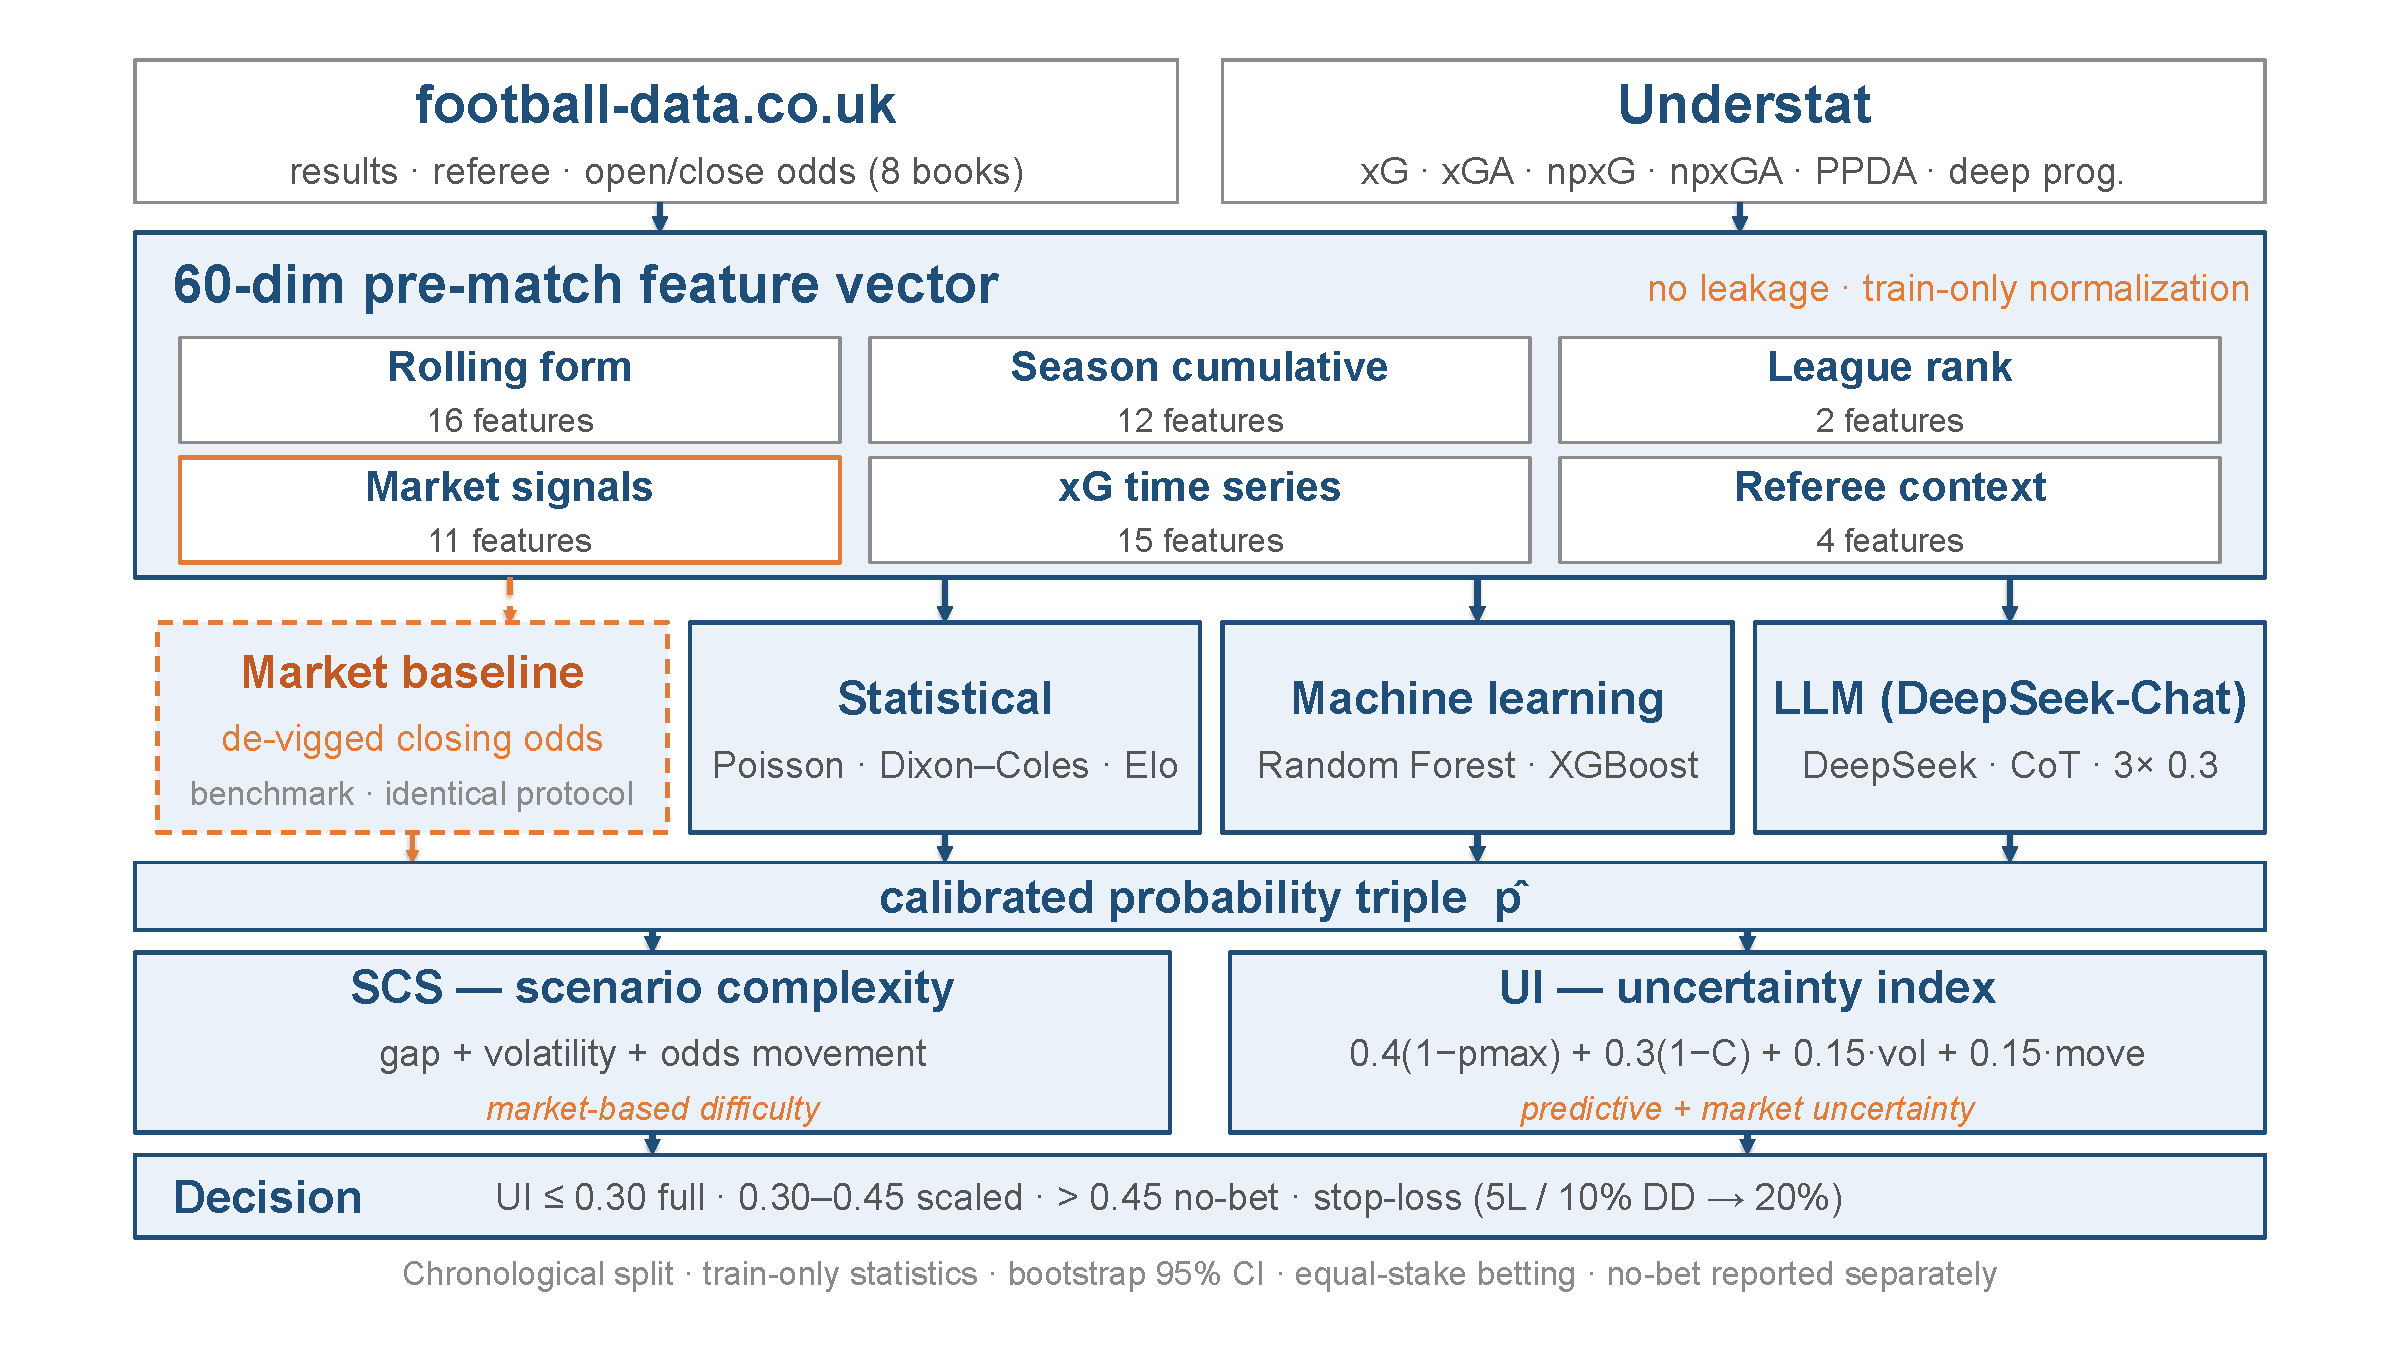
\includegraphics[width=\textwidth]{figures/fig1_framework.pdf}
\caption{Overview of the proposed framework. Historical match data are
converted into a 60-dimensional pre-match feature vector under strict leakage
controls (pre-match cutoff, train-only normalization). Forecast models from
three families produce a calibrated probability triple $\hat{p}$, which is
combined with market-derived signals into two uncertainty scores (SCS, UI).
The decision layer converts these scores into stake sizing and a no-bet
(abstention) rule. The de-vigged closing odds enter twice: as market signals
among the features and as the market baseline under the identical evaluation
protocol.}
\label{fig:framework}
\end{figure}

\begin{figure}[htbp]
\centering
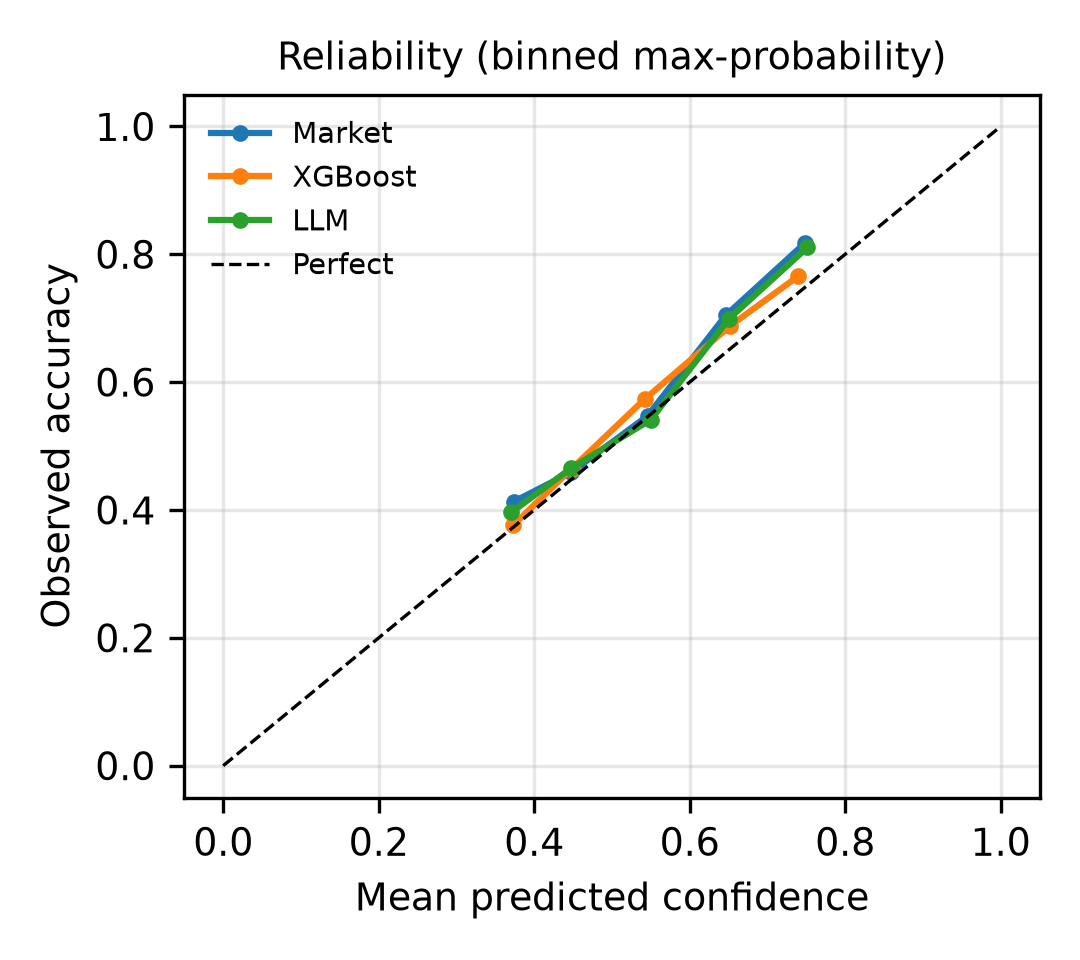
\includegraphics[width=0.9\textwidth]{figures/fig2_reliability.png}
\caption{Reliability diagram (binned max-probability confidence vs.\ observed
accuracy) for the market baseline, XGBoost, and the LLM on the test set.}
\label{fig:reliability}
\end{figure}

\begin{figure}[htbp]
\centering
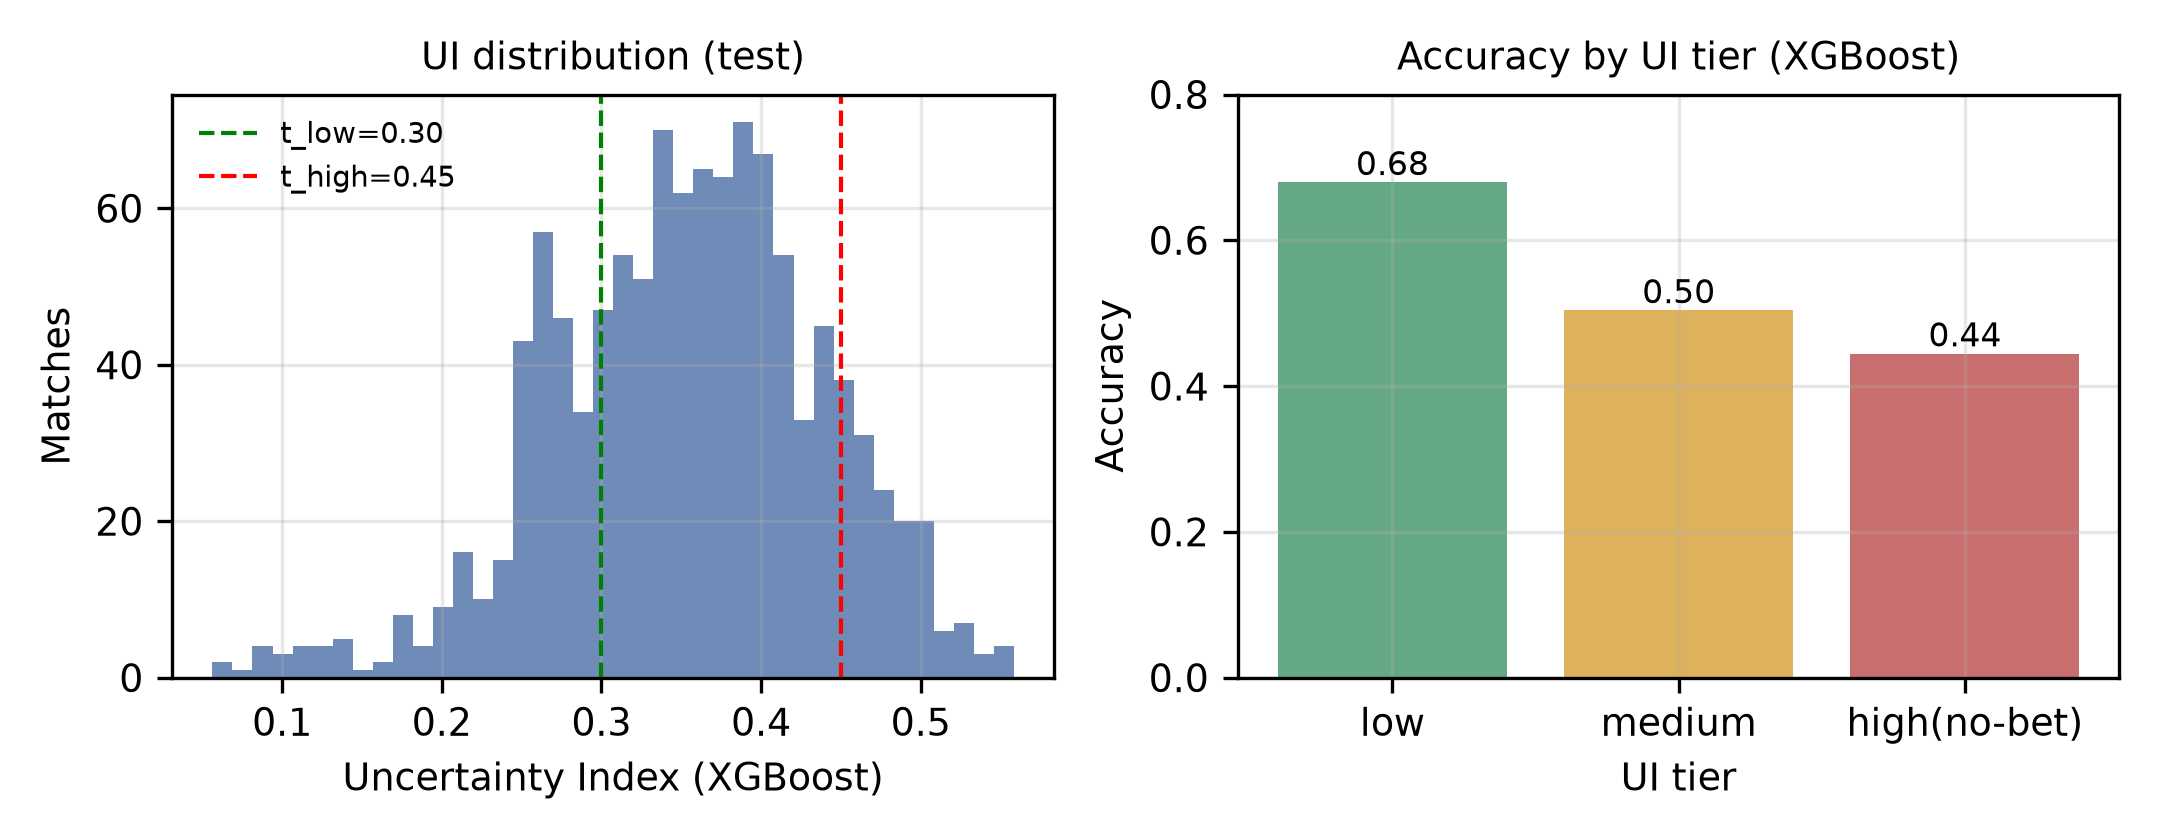
\includegraphics[width=\linewidth]{figures/fig3_ui.png}
\caption{Uncertainty-index distribution (left) and accuracy by UI tier (right)
for XGBoost on the test set.}
\label{fig:ui}
\end{figure}

\begin{figure}[htbp]
\centering
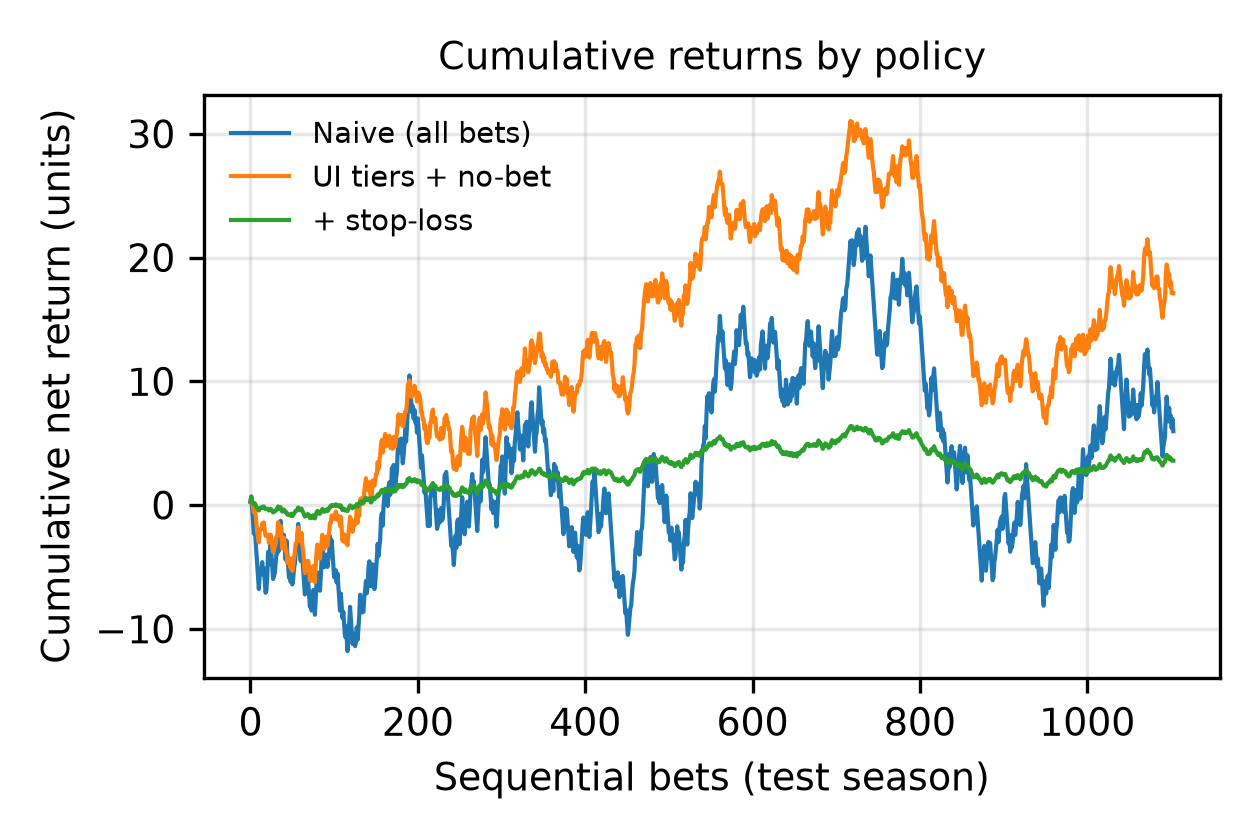
\includegraphics[width=\linewidth]{figures/fig4_roi.png}
\caption{Cumulative net returns of three betting policies on the same XGBoost
probabilities (test period, 1{,}104 matches).}
\label{fig:returns}
\end{figure}

\begin{figure}[htbp]
\centering
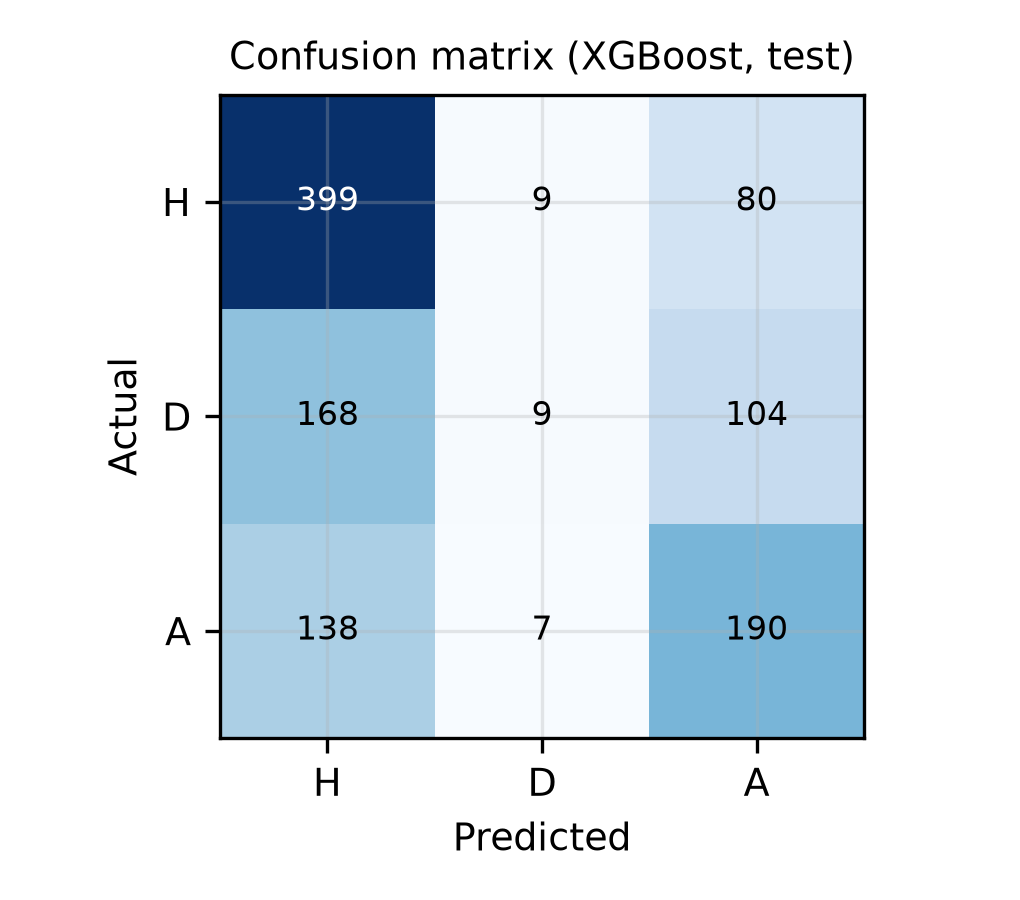
\includegraphics[width=0.75\linewidth]{figures/fig5_confusion.png}
\caption{Confusion matrix of XGBoost on the test set. The draw column is nearly
empty, illustrating systematic under-prediction of draws.}
\label{fig:confusion}
\end{figure}

\begin{figure}[htbp]
\centering
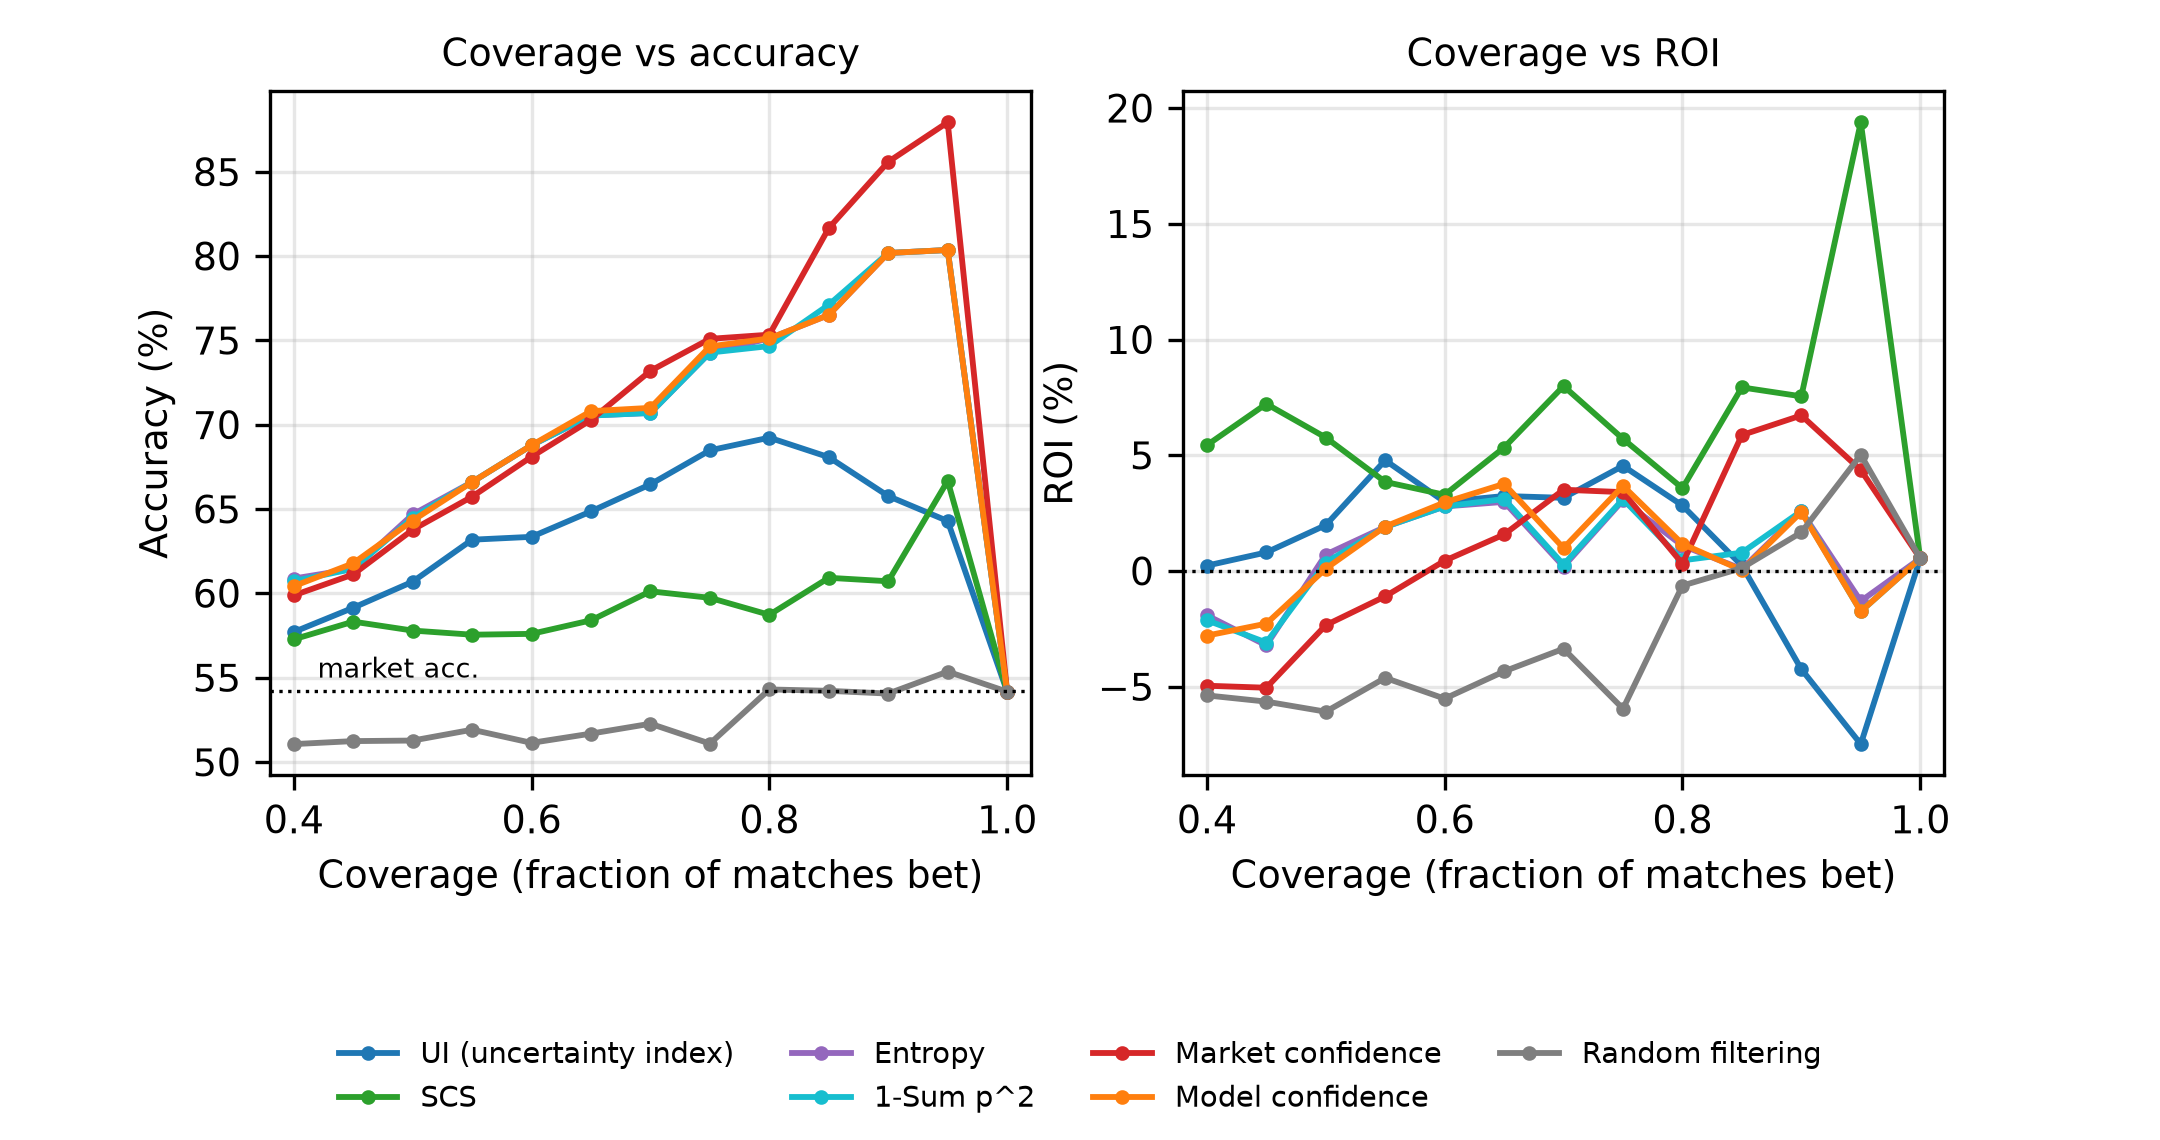
\includegraphics[width=\linewidth]{figures/fig6_coverage.png}
\caption{Coverage--accuracy (left) and coverage--ROI (right) curves for five
no-bet policies on the test period. Market confidence is the strongest accuracy
stratifier but its financial curve is flat to negative at low coverage;
uncertainty-based policies (UI, SCS) trade coverage for ROI without sacrificing
it. Dotted lines mark market accuracy (left) and zero ROI (right).}
\label{fig:coverage}
\end{figure}


% =====================================================================
\section{Discussion}
\label{sec:discussion}

\subsection{Why the market baseline is hard to beat}
The results are consistent with semi-strong market efficiency in football
betting: closing odds aggregate information more accurately than any single
model evaluated here. The 88.3\% share of aggregate permutation importance
carried by market features, the failure of value betting even after
calibration, and the absence of exploitable opening-to-closing drift all point
in the same direction. The practical implication is not that forecasting models
are useless, but that their contribution must be measured in risk-adjusted
terms rather than raw accuracy.

Draws illustrate the point most sharply: the models and the market both
under-predict them by an order of magnitude (2.3\% of matches for XGBoost, 0.3\%
for the market, against an empirical 25.5\%). Outcome predictability is weakest
for this class (Table~\ref{tab:draw}), which is one more reason that difficulty
rather than outcome is what can be predicted.

\subsection{Overconfidence, not information}
The value-betting experiment is instructive: restricting to larger positive EV
made losses worse, and isotonic calibration shrank but did not remove them
(Table~\ref{tab:value}). The model's ``edge'' is concentrated in the region
where it is most confident and most wrong---a signature of overconfidence rather
than information. This contrast---uncertainty filtering helps, confidence-based
selection hurts---is the central practical insight of the paper.

\subsection{Why difficulty is identifiable in an efficient market}
Forecast difficulty has no ground-truth label (Section~\ref{sec:problem-diff}):
the market's probability level and the SCS/UI scores are proxies, checked here
against held-out accuracy and, for the UI, against the market's own probability
level through the conditioning analysis of Section~\ref{sec:rq3}.
Section~\ref{sec:problem-diff} draws the analogy with volatility in financial
forecasting. Efficiency constrains expected returns, not the spread of outcome
uncertainty: match outcomes are unpredictable beyond the market, but how hard a
match is to predict can be established in advance.

The uncertainty index sits on top of this market signal. Its low tier coincides
with strong-market matches (64\% favorites) but is not reducible to market
strength (Section~\ref{sec:rq3}). The mechanism is calibration: the model's
confidence is a calibrated estimate of outcome uncertainty, and the UI combines
it with market-volatility terms that measure how much the market itself
disagrees. Calibrated confidence is a difficulty estimate; raw odds movement is
not.

The no-bet policy bets only where the market, and the model's estimate of it, is
most certain, rather than claiming that the model knows better than the market:
certainty-based filtering helps where confidence-based selection does not
(Table~\ref{tab:value}). The multi-sample consistency term contributes little;
the effective components are predictive confidence and market volatility, both
available at prediction time.

\subsection{Real-world frictions and limitations}
All financial results are gross of transaction costs. Bookmaker margins are
already embedded in the odds settled against, but real-world execution would
add betting taxes, withdrawal fees, and odds slippage---typically 3--7\% of
turnover depending on the jurisdiction. The small positive ROIs observed (up to
1.8\% for the UI-tier strategy) would be entirely consumed by such frictions.
The practical value of the risk-control framework is therefore not
profitability but risk stratification: identifying, in advance, the subset of
matches where even a well-calibrated model is unlikely to be right, so that
capital and attention are directed elsewhere. These results therefore do not
support claims of deployable profitability.

Several further limitations bound the scope of these conclusions. The
text modality is excluded: publicly available news corpora lack
reliable pre-match timestamps at scale, and a rigorous text experiment would
require timestamp-verified article cutoffs (every article checked against
kickoff, undated or post-kickoff articles discarded), protection against
retrieval contamination, and coverage reporting, since news availability varies
across leagues and matches; without them, text features would bring back the
leakage this paper avoids. The held-out period (2025/26 to date) is incomplete and
a few results may move at season end; every number comes from a scripted pipeline,
so the full set can be regenerated then. Financial results rest on one bookmaker's
closing odds and are gross of taxes, so ROI is a decision-quality proxy under
closing-market assumptions rather than deployable profit. The evidence is also
single-sport and single-market: men's football in the five major European leagues.
Other sports, lower divisions or different market structures (Asian handicap,
in-play) are untested, though the mechanism---market efficiency limiting
predictive edge while difficulty stays measurable---is not sport-specific in
principle. The analyses are predictive, not causal, and say nothing about how
odds are formed. Finally, the primary LLM evaluation uses a proprietary API
(DeepSeek-Chat); an open-weight model comparison is additionally reported
(Appendix~\ref{app:llm}).

\subsection{LLM results in context}
The domain-enhanced LLM reaches market-level probability calibration (log loss
0.967 vs.\ 0.967, ECE 0.025 vs.\ 0.026) with no training and no retrieval, at a
cost of \$0.55 for the entire test period. Two qualifications apply:
multi-sample consistency carries no information in this setting
(Section~\ref{sec:llm}), and an open-weight 7B model matches or exceeds the
API model on the same 120-match subset, so the result is not a property of a
specific proprietary model. The LLM contribution is therefore framed as
calibration without training and a cost--performance reference point, not as
predictive superiority.

% =====================================================================
\section{Conclusion}
\label{sec:conclusion}
This paper evaluated football match outcome forecasting without future
information, comparing statistical and tree-based models and a domain-enhanced
LLM against de-vigged closing odds under one counterfactual closing-line
protocol. On 1{,}104 held-out matches no learned method
significantly exceeded market accuracy, and the LLM matched market-level
calibration at low API cost. Feature importance and ablations show that market
signals dominate, referee statistics add nothing measurable, and xG adds a
small consistent gain. The principal positive result is that uncertainty-driven
risk control works: the uncertainty index and corrected scenario-complexity
score stratify held-out matches monotonically, abstention on high-uncertainty
matches improves risk-adjusted returns, and draws are systematically
under-predicted, with class weighting giving a controllable
accuracy--balance trade-off.

These results frame a realistic division of labor for decision-support systems
in sports betting: treat the market as the prior, use models for calibrated
probabilities and explainability, and rely on uncertainty signals---not claimed
accuracy---for risk control. What such a system can realistically deliver in an
efficient market is how likely it is to be wrong, and abstaining on that basis is
the decision-level counterpart of selective prediction. For reproducibility, the
full pipeline and experiment code will be released upon publication; during review
an anonymized copy is available on request.

% =====================================================================
\begin{thebibliography}{21}
\bibitem{halawi2024} D.~Halawi, F.~Zhang, C.~Yueh-Han, and J.~Steinhardt,
``Approaching human-level forecasting with language models,'' \emph{arXiv
preprint arXiv:2402.18563}, 2024.
\bibitem{aia2025} R.~Alur, B.~C.~Stadie, D.~Kang, R.~Chen, M.~McManus,
\emph{et al.}, ``AIA Forecaster: Technical report,'' \emph{arXiv preprint
arXiv:2511.07678}, 2025.
\bibitem{llmprophet2025} Q.~Yang, S.~Mahns, S.~Li, A.~Gu, J.~Wu, and H.~Xu,
``LLM-as-a-prophet: Understanding predictive intelligence with prophet arena,''
\emph{arXiv preprint arXiv:2510.17638}, 2025.
\bibitem{chow1970} C.-K.~Chow, ``On optimum recognition error and reject
tradeoff,'' \emph{IEEE Transactions on Information Theory}, vol.~16, no.~1,
pp.~41--46, 1970.
\bibitem{geifman2017} Y.~Geifman and R.~El-Yaniv, ``Selective classification
for deep neural networks,'' in \emph{Advances in Neural Information Processing
Systems (NeurIPS)}, vol.~30, 2017.
\bibitem{elyaniv2010} R.~El-Yaniv and Y.~Wiener, ``On the foundations of
noise-free selective classification,'' \emph{Journal of Machine Learning
Research}, vol.~11, pp.~1605--1641, 2010.
\bibitem{maher1982} M.~J.~Maher, ``Modelling association football scores,''
\emph{Statistica Neerlandica}, vol.~36, no.~3, pp.~109--118, 1982.
\bibitem{dixoncoles1997} M.~J.~Dixon and S.~G.~Coles, ``Modelling association
football scores and inefficiencies in the football betting market,''
\emph{Journal of the Royal Statistical Society Series C: Applied Statistics},
vol.~46, no.~2, pp.~265--280, 1997.
\bibitem{elo1978} A.~E.~Elo, \emph{The Rating of Chessplayers, Past and
Present}. New York, NY, USA: Arco Publishing, 1978.
\bibitem{hvattum2010} L.~M.~Hvattum and H.~Arntzen, ``Using ELO ratings for
match result prediction in association football,'' \emph{International Journal
of Forecasting}, vol.~26, no.~3, pp.~460--470, 2010.
\bibitem{spann2009} M.~Spann and B.~Skiera, ``Sports forecasting: A comparison
of the forecast accuracy of prediction markets, betting odds and tipsters,''
\emph{Journal of Forecasting}, vol.~28, no.~1, pp.~55--72, 2009.
\bibitem{levitt2004} S.~D.~Levitt, ``Why are gambling markets organised so
differently from financial markets?'' \emph{The Economic Journal}, vol.~114,
no.~495, pp.~223--246, 2004.
\bibitem{franck2010} E.~Franck, E.~Verbeek, and S.~N\"uesch, ``Prediction
accuracy of different market structures: Bookmakers versus a betting
exchange,'' \emph{International Journal of Forecasting}, vol.~26, no.~3,
pp.~448--459, 2010.
\bibitem{decroos2019} T.~Decroos, L.~Bransen, J.~Van~Haaren, and J.~Davis,
``Actions speak louder than goals: Valuing player actions in soccer,'' in
\emph{Proceedings of the 25th ACM SIGKDD International Conference on Knowledge
Discovery \& Data Mining}, 2019, pp.~1851--1861.
\bibitem{robberechts2021} P.~Robberechts, J.~Van~Haaren, and J.~Davis, ``How
data availability affects the ability to learn good xG models,'' in
\emph{Machine Learning and Knowledge Discovery in Databases. Applied Data
Science Track (ECML PKDD 2021)}, LNCS vol.~12977, 2021, pp.~17--32.
\bibitem{guo2017} C.~Guo, G.~Pleiss, Y.~Sun, and K.~Q.~Weinberger, ``On
calibration of modern neural networks,'' in \emph{Proceedings of the 34th
International Conference on Machine Learning (ICML)}, 2017, pp.~1321--1330.
\bibitem{naeini2015} M.~P.~Naeini, G.~Cooper, and M.~Hauskrecht, ``Obtaining
well calibrated probabilities using Bayesian binning into quantiles,'' in
\emph{Proceedings of the 21st ACM SIGKDD International Conference on Knowledge
Discovery and Data Mining}, 2015, pp.~387--396.
\bibitem{kendall2017} A.~Kendall and Y.~Gal, ``What uncertainties do we need in
Bayesian deep learning for computer vision?'' in \emph{Advances in Neural
Information Processing Systems (NeurIPS)}, vol.~30, 2017.
\bibitem{lakshminarayanan2017} B.~Lakshminarayanan, A.~Pritzel, and
C.~Blundell, ``Simple and scalable predictive uncertainty estimation using deep
ensembles,'' in \emph{Advances in Neural Information Processing Systems
(NeurIPS)}, vol.~30, 2017.
\bibitem{ovadia2019} Y.~Ovadia \emph{et al.}, ``Can you trust your model's
uncertainty? Evaluating uncertainty calibration under distributional shifts,''
in \emph{Advances in Neural Information Processing Systems (NeurIPS)},
vol.~32, 2019.
\bibitem{liu2022} G.~Liu, Y.~Luo, O.~Schulte, and P.~Poupart,
``Uncertainty-aware reinforcement learning for risk-sensitive player
evaluation in sports game,'' in \emph{Advances in Neural Information Processing
Systems (NeurIPS)}, vol.~35, 2022.
\end{thebibliography}

% =====================================================================
\appendix
\section*{Appendix}

\section{League and Season Generalization}
\label{app:league}
Table~\ref{tab:league} reports per-league accuracy of the global XGBoost model,
and Table~\ref{tab:lolo} the leave-one-league-out experiment. Performance varies markedly across leagues:
the Bundesliga and La Liga are the most predictable (57.4\% and 57.0\%
accuracy), while the Premier League is the least (50.0\%), the most liquid and
informationally efficient of the five. The leave-one-league-out experiment
shows the same ordering in a stricter setting: a model trained on the other
four leagues degrades most on the Premier League (47.3\%). The ordering is
therefore a property of the competitions rather than of the model.

\begin{table}[H]
\centering
\caption{Per-league performance of the global XGBoost model on the test set.}
\label{tab:league}
\begin{tabular}{lccccc}
\toprule
League & N & Acc & LogLoss & ROI & MDD \\
\midrule
D1 & 188 & 57.4\% & 0.945 & 6.9\% & -6.0\% \\
E0 & 260 & 50.0\% & 1.016 & -7.4\% & -8.1\% \\
F1 & 189 & 55.0\% & 0.953 & 1.1\% & -6.8\% \\
I1 & 239 & 52.7\% & 0.981 & -2.4\% & -7.3\% \\
SP1 & 228 & 57.0\% & 0.947 & 7.0\% & -2.9\% \\
\bottomrule
\end{tabular}
\end{table}

\begin{table}[H]
\centering
\caption{Leave-one-league-out generalization: model trained on the other four
leagues, evaluated on the held-out league (test set).}
\label{tab:lolo}
\small
\begin{tabular}{lcccc}
\toprule
Held-out league & N & Acc & LogLoss & ROI \\
\midrule
E0 & 260 & 47.3\% & 1.015 & -13.5\% \\
D1 & 188 & 54.3\% & 0.942 & -0.9\% \\
F1 & 189 & 55.6\% & 0.958 & 4.5\% \\
I1 & 239 & 53.6\% & 0.979 & 0.6\% \\
SP1 & 228 & 53.5\% & 0.954 & -2.2\% \\
\bottomrule
\end{tabular}
\end{table}

\section{Draw Diagnostics}
\label{app:draw}
Table~\ref{tab:class} reports class-wise metrics for XGBoost on the test set,
and Table~\ref{tab:cost} reports the cost-sensitive training sweep. The
accuracy--balance trade-off is monotone: a draw weight of 1.5 raises macro-F1
from 0.421 to 0.493 and draw recall from 0.032 to 0.356, at the cost of 2.2
points of accuracy.

\begin{table}[H]
\centering
\caption{Class-wise metrics (XGBoost, test set). Empirical draw rate is 25.5\%
but the model predicts a draw in only 2.3\% of matches.}
\label{tab:class}
\small
\begin{tabular}{lcccc}
\toprule
Class & Prec & Recall & F1 & ECE \\
\midrule
Home win & 0.566 & 0.818 & 0.669 & 0.037 \\
Draw & 0.360 & 0.032 & 0.059 & 0.007 \\
Away win & 0.508 & 0.567 & 0.536 & 0.020 \\
\midrule
Pred.\ draw rate & \multicolumn{4}{c}{2.3\%} \\
Empirical draw rate & \multicolumn{4}{c}{25.5\%} \\
\bottomrule
\end{tabular}
\end{table}

\begin{table}[H]
\centering
\caption{Cost-sensitive training: draw class weight sweep (XGBoost, test set).
Weight 1.0 is the baseline.}
\label{tab:cost}
\begin{tabular}{lccccc}
\toprule
$w(\mathrm{draw})$ & Acc & Macro-F1 & Draw R & Draw P & LogLoss \\
\midrule
1.0 & 54.2\% & 0.421 & 0.032 & 0.360 & 0.971 \\
1.5 & 52.0\% & 0.493 & 0.356 & 0.317 & 0.987 \\
2.0 & 46.6\% & 0.456 & 0.584 & 0.300 & 1.012 \\
2.5 & 45.2\% & 0.443 & 0.722 & 0.303 & 1.037 \\
3.0 & 45.6\% & 0.447 & 0.612 & 0.301 & 1.047 \\
\bottomrule
\end{tabular}
\end{table}

\section{Additional Financial Analyses}
\label{app:financial}
Table~\ref{tab:isoton} reports value betting after isotonic calibration (fit on
validation).

\begin{table}[H]
\centering
\caption{Value betting after isotonic calibration (fit on validation). Losses
shrink but remain negative: calibration cannot create information the model
does not have.}
\label{tab:isoton}
\small
\begin{tabular}{lcccc}
\toprule
EV thresh. & ROI & N bets & Coverage \\
\midrule
0.00 & -7.1\% & 965 & 87.4\% \\
0.02 & -5.3\% & 876 & 79.3\% \\
0.05 & -7.0\% & 724 & 65.6\% \\
0.08 & -7.7\% & 574 & 52.0\% \\
0.10 & -7.5\% & 484 & 43.8\% \\
\bottomrule
\end{tabular}
\end{table}

\section{Uncertainty Tiers: Additional Scores and Models}
\label{app:unc}
Table~\ref{tab:scs} splits the test set by the scenario-complexity score, and
Table~\ref{tab:uillm} replicates the UI stratification for the LLM. The
monotone pattern is a property of the task and the features, not of a
particular model.

\begin{table}[H]
\centering
\caption{Scenario-complexity tiers (XGBoost, test set, thresholds 1.4/1.8).
Higher SCS indicates harder matches.}
\label{tab:scs}
\small
\begin{tabular}{lccc}
\toprule
SCS tier & N & Acc & ROI \\
\midrule
low (SCS $\le$ 1.4) & 246 & 58.9\% & 5.1\% \\
mid (1.4 $<$ SCS $\le$ 1.8) & 356 & 57.3\% & 7.0\% \\
high (SCS $>$ 1.8) & 502 & 49.6\% & -6.3\% \\
\bottomrule
\end{tabular}
\end{table}

\begin{table}[H]
\centering
\caption{Uncertainty-index tiers for the LLM (test set). The same
stratification pattern replicates across model families.}
\label{tab:uillm}
\small
\begin{tabular}{lcccc}
\toprule
UI tier & N & Acc & ROI & MDD \\
\midrule
low & 259 & 68.7\% & 3.2\% & -4.4\% \\
medium & 689 & 49.8\% & -0.7\% & -4.5\% \\
high (no-bet) & 156 & 47.4\% & -9.6\% & -13.8\% \\
\bottomrule
\end{tabular}
\end{table}

\section{LLM Diagnostics}
\label{app:llm}
Table~\ref{tab:temp} reports temperature sensitivity, and
Table~\ref{tab:llmcmp} compares the API chat model with an open-weight local
model and a reasoning model on the same first 120 test-set matches. This
comparison is robustness evidence only: the sample is small and confidence
intervals overlap, so no superiority claim is made for any model.

\begin{table}[H]
\centering
\caption{Temperature sensitivity (same 120 matches). Multi-sample consistency
remains near 1.0 at both temperatures and does not correlate with correctness.}
\label{tab:temp}
\begin{tabular}{lcccccc}
\toprule
Config & Acc & LogLoss & ECE & Cons. & $r$(cons, corr) \\
\midrule
DeepSeek $t=0.3$ & 54.2\% & 0.927 & 0.097 & 0.995 & -0.068 \\
DeepSeek $t=0.7$ & 55.0\% & 0.927 & 0.089 & 0.990 & 0.037 \\
\bottomrule
\end{tabular}
\end{table}

\begin{table}[H]
\centering
\caption{LLM model comparison on the same first 120 test-set matches:
DeepSeek-Chat and the local Qwen with 3 samples each, DeepSeek-Reasoner with 1
sample (reasoning models are roughly an order of magnitude slower; runtime
constraint).}
\label{tab:llmcmp}
\begin{tabular}{lcccccc}
\toprule
Model & Acc & LogLoss & ECE & ROI & Win rate \\
\midrule
DeepSeek-Chat (API) & 54.2\% & 0.927 & 0.097 & -5.5\% & 54.2\% \\
DeepSeek-Reasoner (API) & 55.2\% & 0.906 & 0.090 & -4.4\% & 55.2\% \\
Qwen2.5-Coder-7B (local) & 57.5\% & 0.915 & 0.081 & 3.6\% & 57.5\% \\
\bottomrule
\end{tabular}
\end{table}

\end{document}
